\documentclass[11pt,a4paper]{article}

% Packages
\usepackage[utf8]{inputenc}
\usepackage[T1]{fontenc}
\usepackage[margin=2.5cm]{geometry}
\usepackage{graphicx}
\usepackage{xcolor}
\usepackage{tikz}
\usetikzlibrary{shapes.geometric, arrows.meta, positioning, calc, fit, backgrounds, decorations.pathreplacing, shadows}
\usepackage{pgfplots}
\pgfplotsset{compat=1.18}
\usepackage{listings}
\usepackage{hyperref}
\usepackage{booktabs}
\usepackage{longtable}
\usepackage{enumitem}
\usepackage{fancyhdr}
\usepackage{titlesec}
\usepackage{tocloft}
\usepackage{amsmath}
\usepackage{amssymb}
\usepackage{float}
\usepackage{subcaption}
\usepackage{tcolorbox}

% Colors
\definecolor{primary}{RGB}{41, 128, 185}
\definecolor{secondary}{RGB}{52, 73, 94}
\definecolor{accent}{RGB}{231, 76, 60}
\definecolor{success}{RGB}{39, 174, 96}
\definecolor{warning}{RGB}{241, 196, 15}
\definecolor{codebackground}{RGB}{248, 248, 248}
\definecolor{codeborder}{RGB}{200, 200, 200}

% TikZ styles
\tikzstyle{component} = [rectangle, rounded corners, minimum width=3cm, minimum height=1cm, text centered, draw=primary, fill=primary!10, font=\small]
\tikzstyle{server} = [rectangle, rounded corners, minimum width=2.5cm, minimum height=0.8cm, text centered, draw=success, fill=success!10, font=\small]
\tikzstyle{client} = [rectangle, rounded corners, minimum width=2.5cm, minimum height=0.8cm, text centered, draw=accent, fill=accent!10, font=\small]
\tikzstyle{monitor} = [rectangle, rounded corners, minimum width=2.5cm, minimum height=0.8cm, text centered, draw=warning, fill=warning!10, font=\small]
\tikzstyle{arrow} = [thick,->,>=Stealth]
\tikzstyle{biarrow} = [thick,<->,>=Stealth]
\tikzstyle{dashedarrow} = [thick,->,>=Stealth,dashed]
\tikzstyle{container} = [rectangle, draw=secondary, dashed, inner sep=10pt]

% Code listing style
\lstdefinestyle{yaml}{
    backgroundcolor=\color{codebackground},
    basicstyle=\ttfamily\footnotesize,
    breakatwhitespace=false,
    breaklines=true,
    captionpos=b,
    commentstyle=\color{gray},
    frame=single,
    keepspaces=true,
    keywordstyle=\color{primary}\bfseries,
    numbers=left,
    numbersep=5pt,
    numberstyle=\tiny\color{gray},
    rulecolor=\color{codeborder},
    showspaces=false,
    showstringspaces=false,
    showtabs=false,
    stringstyle=\color{success},
    tabsize=2,
}

\lstdefinestyle{python}{
    backgroundcolor=\color{codebackground},
    basicstyle=\ttfamily\footnotesize,
    breakatwhitespace=false,
    breaklines=true,
    captionpos=b,
    commentstyle=\color{gray}\itshape,
    frame=single,
    keepspaces=true,
    keywordstyle=\color{primary}\bfseries,
    language=Python,
    numbers=left,
    numbersep=5pt,
    numberstyle=\tiny\color{gray},
    rulecolor=\color{codeborder},
    showspaces=false,
    showstringspaces=false,
    showtabs=false,
    stringstyle=\color{success},
    tabsize=4,
}

\lstdefinestyle{bash}{
    backgroundcolor=\color{codebackground},
    basicstyle=\ttfamily\footnotesize,
    breakatwhitespace=false,
    breaklines=true,
    captionpos=b,
    commentstyle=\color{gray},
    frame=single,
    keepspaces=true,
    keywordstyle=\color{primary}\bfseries,
    language=bash,
    numbers=none,
    rulecolor=\color{codeborder},
    showspaces=false,
    showstringspaces=false,
    showtabs=false,
    stringstyle=\color{success},
    tabsize=2,
}

% Placeholder box
\newtcolorbox{placeholder}[1][]{
    colback=yellow!20,
    colframe=orange!75!black,
    fonttitle=\bfseries,
    title={PLACEHOLDER: #1},
    sharp corners,
    boxrule=2pt
}

% Header and footer
\pagestyle{fancy}
\fancyhf{}
\fancyhead[L]{\leftmark}
\fancyhead[R]{HPC Benchmark Toolkit}
\fancyfoot[C]{\thepage}
\renewcommand{\headrulewidth}{0.4pt}
\renewcommand{\footrulewidth}{0.4pt}

% Hyperref setup
\hypersetup{
    colorlinks=true,
    linkcolor=primary,
    filecolor=accent,
    urlcolor=primary,
    citecolor=success,
}

% Title formatting
\titleformat{\section}
{\normalfont\Large\bfseries\color{primary}}{\thesection}{1em}{}
\titleformat{\subsection}
{\normalfont\large\bfseries\color{secondary}}{\thesubsection}{1em}{}
\titleformat{\subsubsection}
{\normalfont\normalsize\bfseries\color{secondary}}{\thesubsubsection}{1em}{}

\begin{document}

% Title Page
\begin{titlepage}
    \centering
    \vspace*{2cm}

    {\Huge\bfseries HPC Benchmark Toolkit\\[0.5cm]}
    {\Large\itshape Technical Report\\[1cm]}

    \vspace{2cm}

    {\Large A Comprehensive Framework for Benchmarking\\LLM Inference Services on HPC Clusters\\[1cm]}

    \vfill

    {\large
    \begin{tabular}{ll}
        \textbf{Target Platform:} & MeluXina HPC Cluster \\
        \textbf{Container Runtime:} & Apptainer/Singularity \\
        \textbf{Scheduler:} & Slurm \\
        \textbf{Services:} & Ollama, vLLM (Single \& Distributed) \\
    \end{tabular}
    }

    \vspace{2cm}

    {\large January 2025}
\end{titlepage}

% Table of Contents
\tableofcontents
\newpage

% ============================================================================
\section{Introduction}
% ============================================================================

\subsection{Project Overview}

The HPC Benchmark Toolkit is a production-ready framework designed for benchmarking Large Language Model (LLM) inference services on High-Performance Computing (HPC) clusters. The toolkit addresses the critical need for reproducible, scalable, and observable benchmarking in enterprise AI deployments.

\subsubsection{Motivation}

Modern AI deployments require careful performance characterization before production rollout. Key challenges include:

\begin{itemize}
    \item \textbf{Reproducibility}: Experiments must be repeatable with identical configurations
    \item \textbf{Scalability}: Benchmarks must scale from single-node to multi-node distributed setups
    \item \textbf{Observability}: Real-time metrics are essential for performance analysis
    \item \textbf{HPC Integration}: Seamless integration with Slurm and containerized workloads
\end{itemize}

\subsubsection{Key Features}

\begin{table}[H]
\centering
\begin{tabular}{@{}lp{10cm}@{}}
\toprule
\textbf{Feature} & \textbf{Description} \\
\midrule
Multi-Service Support & Ollama, vLLM (single and distributed), extensible architecture \\
Distributed Benchmarking & Multi-node server/client orchestration with Ray \\
Real-Time Monitoring & Prometheus/Grafana integration with live dashboards \\
Recipe-Driven & YAML configurations for reproducible experiments \\
HPC-Optimized & Slurm integration, Apptainer container support \\
Comprehensive Metrics & Latency (p50/p90/p99), throughput, resource utilization \\
\bottomrule
\end{tabular}
\caption{Key features of the HPC Benchmark Toolkit}
\end{table}

\subsection{Supported Services}

The toolkit currently supports the following inference services:

\begin{table}[H]
\centering
\begin{tabular}{@{}llll@{}}
\toprule
\textbf{Service} & \textbf{Description} & \textbf{Default Port} & \textbf{API Type} \\
\midrule
Ollama & Local LLM inference server & 11434 & REST \\
vLLM & High-throughput LLM serving & 8000 & OpenAI-compatible \\
vLLM Distributed & Multi-node vLLM with Ray & 8000 & OpenAI-compatible \\
Dummy & Template for custom services & 5000 & REST \\
\bottomrule
\end{tabular}
\caption{Supported inference services}
\end{table}

% ============================================================================
\section{System Architecture}
% ============================================================================

\subsection{High-Level Architecture}

The system follows a modular architecture with clear separation of concerns. Figure~\ref{fig:high-level-arch} illustrates the high-level component structure.

\begin{figure}[H]
\centering
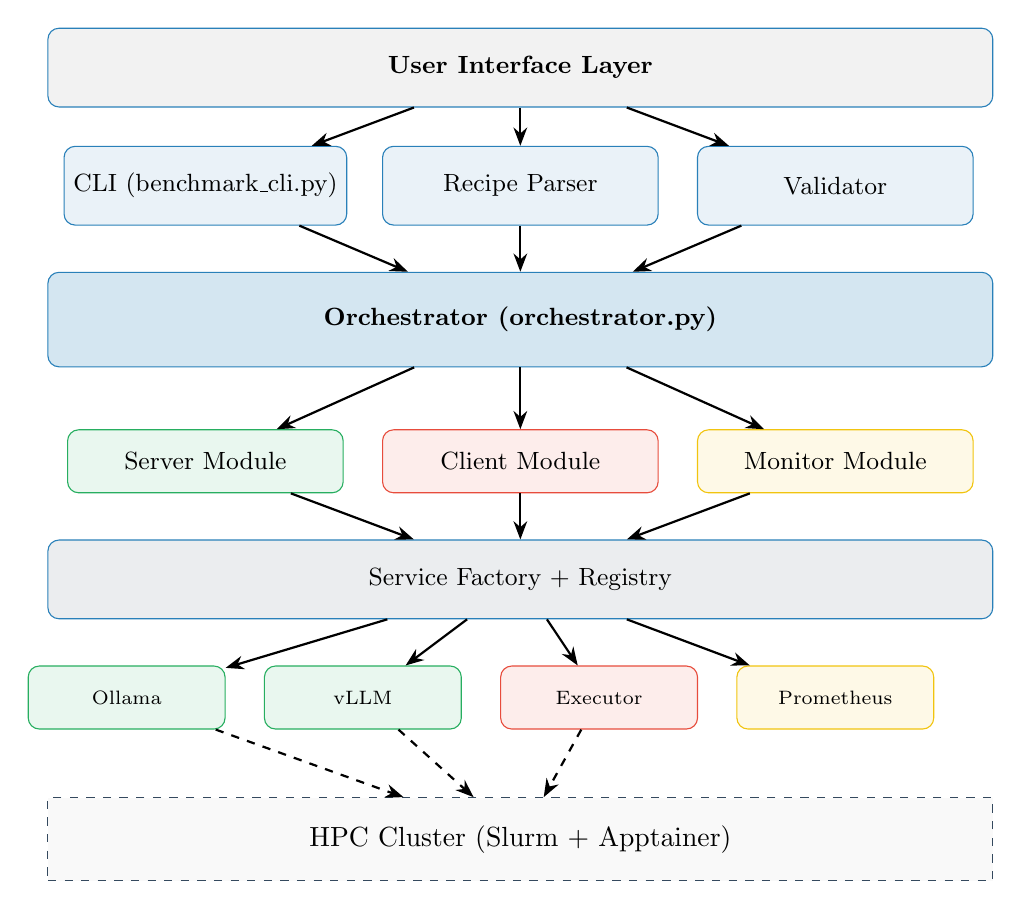
\begin{tikzpicture}[node distance=1.5cm and 2cm]
    % User layer
    \node[component, minimum width=12cm, fill=gray!10] (user) at (0, 5) {\textbf{User Interface Layer}};

    % Interface components
    \node[component, minimum width=3.5cm] (cli) at (-4, 3.5) {CLI (benchmark\_cli.py)};
    \node[component, minimum width=3.5cm] (recipe) at (0, 3.5) {Recipe Parser};
    \node[component, minimum width=3.5cm] (validator) at (4, 3.5) {Validator};

    % Orchestrator
    \node[component, minimum width=12cm, minimum height=1.2cm, fill=primary!20] (orch) at (0, 1.8) {\textbf{Orchestrator (orchestrator.py)}};

    % Core modules
    \node[server, minimum width=3.5cm] (servers) at (-4, 0) {Server Module};
    \node[client, minimum width=3.5cm] (clients) at (0, 0) {Client Module};
    \node[monitor, minimum width=3.5cm] (monitors) at (4, 0) {Monitor Module};

    % Service Factory
    \node[component, minimum width=12cm, fill=secondary!10] (factory) at (0, -1.5) {Service Factory + Registry};

    % Implementations
    \node[server, minimum width=2.5cm, font=\scriptsize] (ollama) at (-5, -3) {Ollama};
    \node[server, minimum width=2.5cm, font=\scriptsize] (vllm) at (-2, -3) {vLLM};
    \node[client, minimum width=2.5cm, font=\scriptsize] (exec1) at (1, -3) {Executor};
    \node[monitor, minimum width=2.5cm, font=\scriptsize] (prom) at (4, -3) {Prometheus};

    % Cluster layer
    \node[container, minimum width=12cm, minimum height=1cm, fill=gray!5] (cluster) at (0, -4.8) {HPC Cluster (Slurm + Apptainer)};

    % Arrows
    \draw[arrow] (user) -- (cli);
    \draw[arrow] (user) -- (recipe);
    \draw[arrow] (user) -- (validator);
    \draw[arrow] (cli) -- (orch);
    \draw[arrow] (recipe) -- (orch);
    \draw[arrow] (validator) -- (orch);
    \draw[arrow] (orch) -- (servers);
    \draw[arrow] (orch) -- (clients);
    \draw[arrow] (orch) -- (monitors);
    \draw[arrow] (servers) -- (factory);
    \draw[arrow] (clients) -- (factory);
    \draw[arrow] (monitors) -- (factory);
    \draw[arrow] (factory) -- (ollama);
    \draw[arrow] (factory) -- (vllm);
    \draw[arrow] (factory) -- (exec1);
    \draw[arrow] (factory) -- (prom);
    \draw[dashedarrow] (ollama) -- (cluster);
    \draw[dashedarrow] (vllm) -- (cluster);
    \draw[dashedarrow] (exec1) -- (cluster);
\end{tikzpicture}
\caption{High-level system architecture}
\label{fig:high-level-arch}
\end{figure}

\subsection{Design Patterns}

The toolkit employs several software design patterns to ensure maintainability and extensibility:

\subsubsection{Factory Pattern}

The \texttt{ServiceFactory} class provides dynamic component instantiation based on service type:

\begin{lstlisting}[style=python, caption={ServiceFactory implementation pattern}]
class ServiceFactory:
    _registry = {}

    @classmethod
    def register_service(cls, name, server_cls, controller_cls, executor_cls):
        cls._registry[name] = {
            'server': server_cls,
            'controller': controller_cls,
            'executor': executor_cls
        }

    @classmethod
    def create_server_manager(cls, service_name, config):
        return cls._registry[service_name]['server'](config)
\end{lstlisting}

\subsubsection{Template Method Pattern}

Base classes define algorithm skeletons while subclasses provide specific implementations:

\begin{figure}[H]
\centering
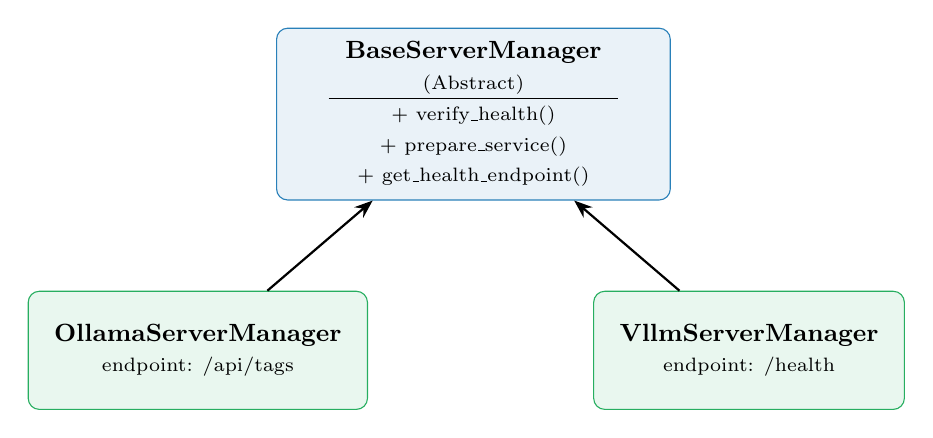
\begin{tikzpicture}[node distance=2cm]
    % Base class
    \node[component, minimum width=5cm, minimum height=2cm] (base) at (0, 2) {
        \begin{tabular}{c}
            \textbf{BaseServerManager} \\
            \scriptsize (Abstract) \\
            \hline
            \scriptsize + verify\_health() \\
            \scriptsize + prepare\_service() \\
            \scriptsize + get\_health\_endpoint()
        \end{tabular}
    };

    % Concrete classes
    \node[server, minimum width=3.5cm, minimum height=1.5cm] (ollama) at (-3.5, -1) {
        \begin{tabular}{c}
            \textbf{OllamaServerManager} \\
            \scriptsize endpoint: /api/tags
        \end{tabular}
    };

    \node[server, minimum width=3.5cm, minimum height=1.5cm] (vllm) at (3.5, -1) {
        \begin{tabular}{c}
            \textbf{VllmServerManager} \\
            \scriptsize endpoint: /health
        \end{tabular}
    };

    % Inheritance arrows
    \draw[arrow] (ollama) -- (base);
    \draw[arrow] (vllm) -- (base);
\end{tikzpicture}
\caption{Template Method Pattern in Server Managers}
\end{figure}

\subsection{Component Details}

\subsubsection{Server Managers}

Server managers handle the lifecycle of inference services:

\begin{itemize}
    \item \textbf{Health Checking}: Polls service endpoints to verify readiness
    \item \textbf{Service Preparation}: Loads models, initializes resources
    \item \textbf{Configuration Parsing}: Extracts service-specific settings from recipes
\end{itemize}

\begin{table}[H]
\centering
\begin{tabular}{@{}llll@{}}
\toprule
\textbf{Manager} & \textbf{Health Endpoint} & \textbf{Port} & \textbf{Special Features} \\
\midrule
OllamaServerManager & /api/tags & 11434 & Model pulling via /api/pull \\
VllmServerManager & /health & 8000 & Ray cluster integration \\
DummyServerManager & /health & 5000 & Template implementation \\
\bottomrule
\end{tabular}
\caption{Server Manager implementations}
\end{table}

\subsubsection{Workload Controllers}

Controllers coordinate workload execution across client nodes:

\begin{figure}[H]
\centering
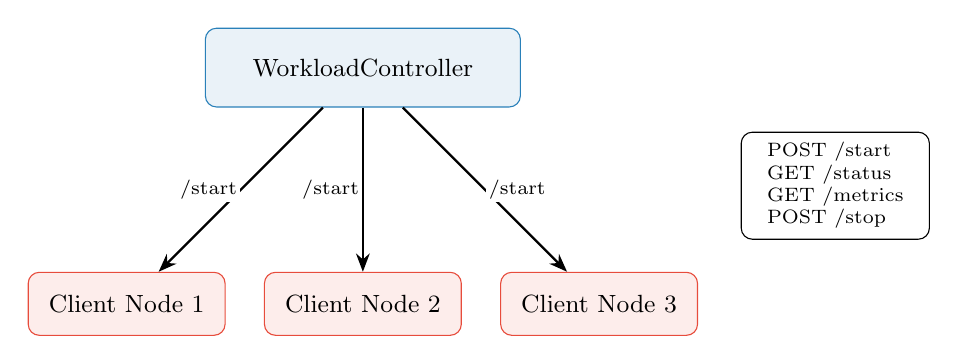
\begin{tikzpicture}[node distance=1.5cm]
    % Controller
    \node[component, minimum width=4cm] (ctrl) at (0, 3) {WorkloadController};

    % Client nodes
    \node[client, minimum width=2.5cm] (c1) at (-3, 0) {Client Node 1};
    \node[client, minimum width=2.5cm] (c2) at (0, 0) {Client Node 2};
    \node[client, minimum width=2.5cm] (c3) at (3, 0) {Client Node 3};

    % Arrows with methods
    \draw[arrow] (ctrl) -- node[left, font=\scriptsize, fill=white, inner sep=1pt] {/start} (c1);
    \draw[arrow] (ctrl) -- node[left, font=\scriptsize, fill=white, inner sep=1pt] {/start} (c2);
    \draw[arrow] (ctrl) -- node[right, font=\scriptsize, fill=white, inner sep=1pt] {/start} (c3);

    % Method list
    \node[draw, rounded corners, fill=white, font=\scriptsize] at (6, 1.5) {
        \begin{tabular}{l}
            POST /start \\
            GET /status \\
            GET /metrics \\
            POST /stop
        \end{tabular}
    };
\end{tikzpicture}
\caption{Workload Controller to Client communication}
\end{figure}

\subsubsection{Workload Executors}

Executors run on client nodes as Flask servers, executing the actual benchmark workload:

\begin{lstlisting}[style=python, caption={Workload Executor REST API}]
# Flask endpoints exposed by each executor
GET  /health              # Check executor status
POST /start               # Start workload with JSON config
GET  /status              # Get current workload status
GET  /metrics             # Fetch collected metrics
GET  /metrics/prometheus  # Prometheus-compatible format
POST /stop                # Stop workload execution
\end{lstlisting}

% ============================================================================
\section{Communication Architecture}
% ============================================================================

\subsection{Overview}

The toolkit employs a hybrid communication architecture combining:
\begin{itemize}
    \item \textbf{REST/HTTP}: Control plane communication between orchestrator and components
    \item \textbf{Service APIs}: Data plane communication between clients and inference servers
    \item \textbf{Prometheus Push/Pull}: Metrics collection and aggregation
\end{itemize}

\subsection{Control Plane Communication}

\begin{figure}[H]
\centering
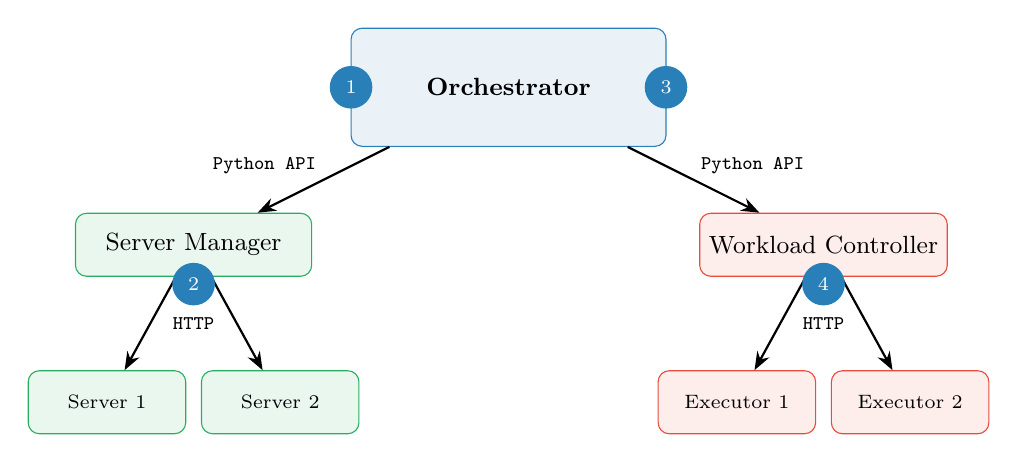
\begin{tikzpicture}[node distance=2cm]
    % Orchestrator
    \node[component, minimum width=4cm, minimum height=1.5cm] (orch) at (0, 4) {\textbf{Orchestrator}};

    % Server Manager
    \node[server, minimum width=3cm] (sm) at (-4, 2) {Server Manager};

    % Workload Controller
    \node[client, minimum width=3cm] (wc) at (4, 2) {Workload Controller};

    % Server nodes
    \node[server, minimum width=2cm, font=\scriptsize] (s1) at (-5.1, 0) {Server 1};
    \node[server, minimum width=2cm, font=\scriptsize] (s2) at (-2.9, 0) {Server 2};

    % Client executors
    \node[client, minimum width=2cm, font=\scriptsize] (e1) at (2.9, 0) {Executor 1};
    \node[client, minimum width=2cm, font=\scriptsize] (e2) at (5.1, 0) {Executor 2};

    % Protocol labels
    \node[fill=white, font=\scriptsize\ttfamily] at (-3.1, 3) {Python API};
    \node[fill=white, font=\scriptsize\ttfamily] at (3.1, 3) {Python API};
    \node[fill=white, font=\scriptsize\ttfamily] at (-4, 1) {HTTP};
    \node[fill=white, font=\scriptsize\ttfamily] at (4, 1) {HTTP};

    % Arrows
    \draw[arrow] (orch) -- (sm);
    \draw[arrow] (orch) -- (wc);
    \draw[arrow] (sm) -- (s1);
    \draw[arrow] (sm) -- (s2);
    \draw[arrow] (wc) -- (e1);
    \draw[arrow] (wc) -- (e2);

    % Sequence numbers
    \node[circle, fill=primary, text=white, font=\scriptsize] at (-2, 4) {1};
    \node[circle, fill=primary, text=white, font=\scriptsize] at (-4, 1.5) {2};
    \node[circle, fill=primary, text=white, font=\scriptsize] at (2, 4) {3};
    \node[circle, fill=primary, text=white, font=\scriptsize] at (4, 1.5) {4};
\end{tikzpicture}
\caption{Control plane communication flow}
\label{fig:control-plane}
\end{figure}

\subsection{Data Plane Communication}

During benchmark execution, clients send inference requests directly to servers:

\begin{figure}[H]
\centering
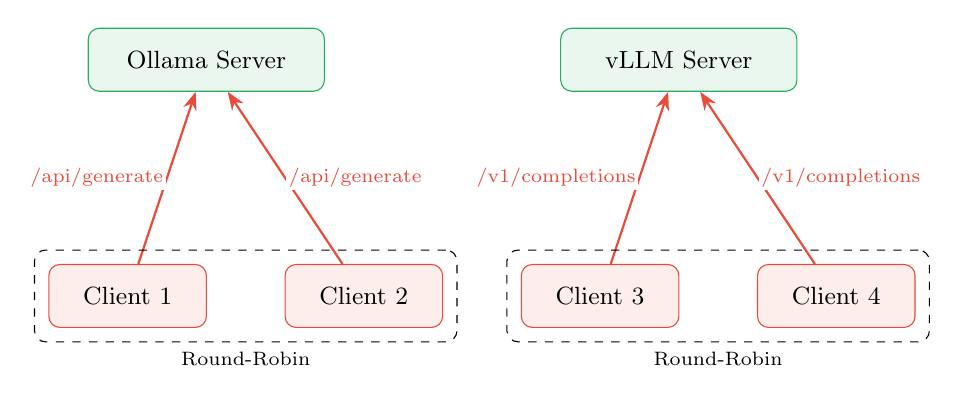
\begin{tikzpicture}[node distance=2cm]
    % Servers
    \node[server, minimum width=3cm] (s1) at (-3, 2) {Ollama Server};
    \node[server, minimum width=3cm] (s2) at (3, 2) {vLLM Server};

    % Clients
    \node[client, minimum width=2cm] (c1) at (-4, -1) {Client 1};
    \node[client, minimum width=2cm] (c2) at (-1, -1) {Client 2};
    \node[client, minimum width=2cm] (c3) at (2, -1) {Client 3};
    \node[client, minimum width=2cm] (c4) at (5, -1) {Client 4};

    % Request arrows
    \draw[arrow, accent] (c1) -- node[left, font=\scriptsize, fill=white, inner sep=1pt] {/api/generate} (s1);
    \draw[arrow, accent] (c2) -- node[right, font=\scriptsize, fill=white, inner sep=1pt] {/api/generate} (s1);
    \draw[arrow, accent] (c3) -- node[left, font=\scriptsize, fill=white, inner sep=1pt] {/v1/completions} (s2);
    \draw[arrow, accent] (c4) -- node[right, font=\scriptsize, fill=white, inner sep=1pt] {/v1/completions} (s2);

    % Load distribution label
    \node[draw, dashed, rounded corners, fit=(c1)(c2), inner sep=5pt, label=below:{\scriptsize Round-Robin}] {};
    \node[draw, dashed, rounded corners, fit=(c3)(c4), inner sep=5pt, label=below:{\scriptsize Round-Robin}] {};
\end{tikzpicture}
\caption{Data plane: Client to Server inference requests}
\end{figure}

\subsection{Metrics Collection Pipeline}

\begin{figure}[H]
\centering
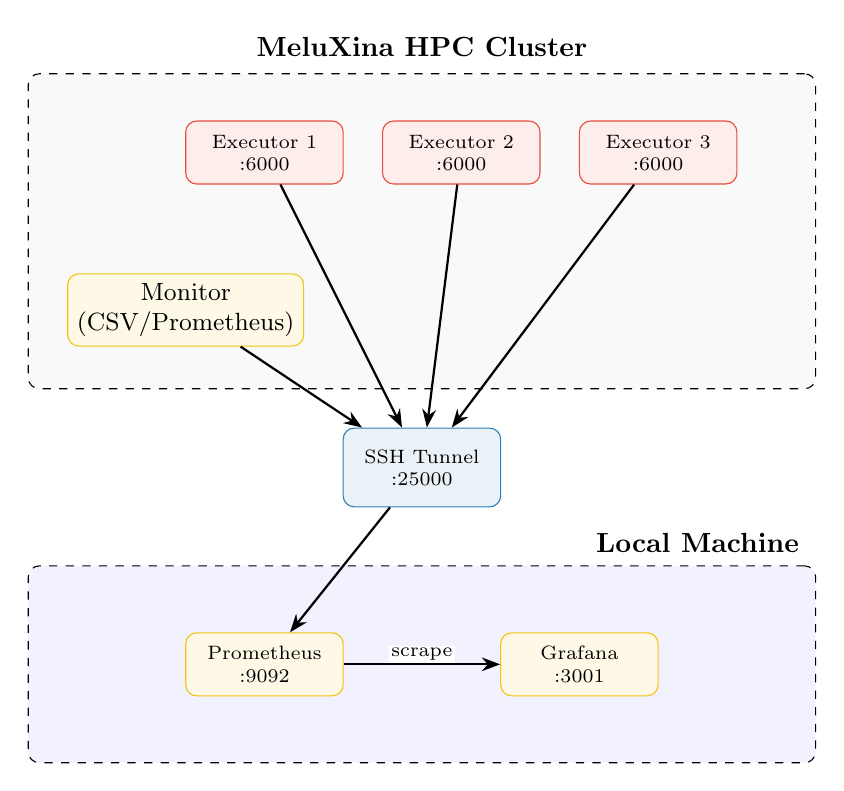
\begin{tikzpicture}[node distance=1.5cm]
    % HPC Cluster boundary
    \begin{scope}[on background layer]
        \node[draw, dashed, rounded corners, minimum width=10cm, minimum height=4cm, fill=gray!5] (hpc) at (0, 2) {};
        \node[above] at (0, 4.1) {\textbf{MeluXina HPC Cluster}};
    \end{scope}

    % Executors
    \node[client, minimum width=2cm, font=\scriptsize, align=center] (e1) at (-2, 3) {Executor 1\\:6000};
    \node[client, minimum width=2cm, font=\scriptsize, align=center] (e2) at (0.5, 3) {Executor 2\\:6000};
    \node[client, minimum width=2cm, font=\scriptsize, align=center] (e3) at (3, 3) {Executor 3\\:6000};

    % Monitor
    \node[monitor, minimum width=2.5cm, align=center] (mon) at (-3, 1) {Monitor\\(CSV/Prometheus)};

    % SSH Tunnel
    \node[component, minimum width=2cm, font=\scriptsize, align=center] (tunnel) at (0, -1) {SSH Tunnel\\:25000};

    % Laptop boundary
    \begin{scope}[on background layer]
        \node[draw, dashed, rounded corners, minimum width=10cm, minimum height=2.5cm, fill=blue!5] (laptop) at (0, -3.5) {};
        \node[above] at (3.5, -2.2) {\textbf{Local Machine}};
    \end{scope}

    % Prometheus & Grafana
    \node[monitor, minimum width=2cm, font=\scriptsize, align=center] (prom) at (-2, -3.5) {Prometheus\\:9092};
    \node[monitor, minimum width=2cm, font=\scriptsize, align=center] (grafana) at (2, -3.5) {Grafana\\:3001};

    % Arrows
    \draw[arrow] (e1) -- (tunnel);
    \draw[arrow] (e2) -- (tunnel);
    \draw[arrow] (e3) -- (tunnel);
    \draw[arrow] (mon) -- (tunnel);
    \draw[arrow] (tunnel) -- (prom);
    \draw[arrow] (prom) -- node[above, font=\scriptsize, fill=white, inner sep=1pt] {scrape} (grafana);

\end{tikzpicture}
\caption{Metrics collection pipeline with SSH tunneling}
\label{fig:metrics-pipeline}
\end{figure}

\subsection{Message Sequence Diagram}

\begin{figure}[H]
\centering
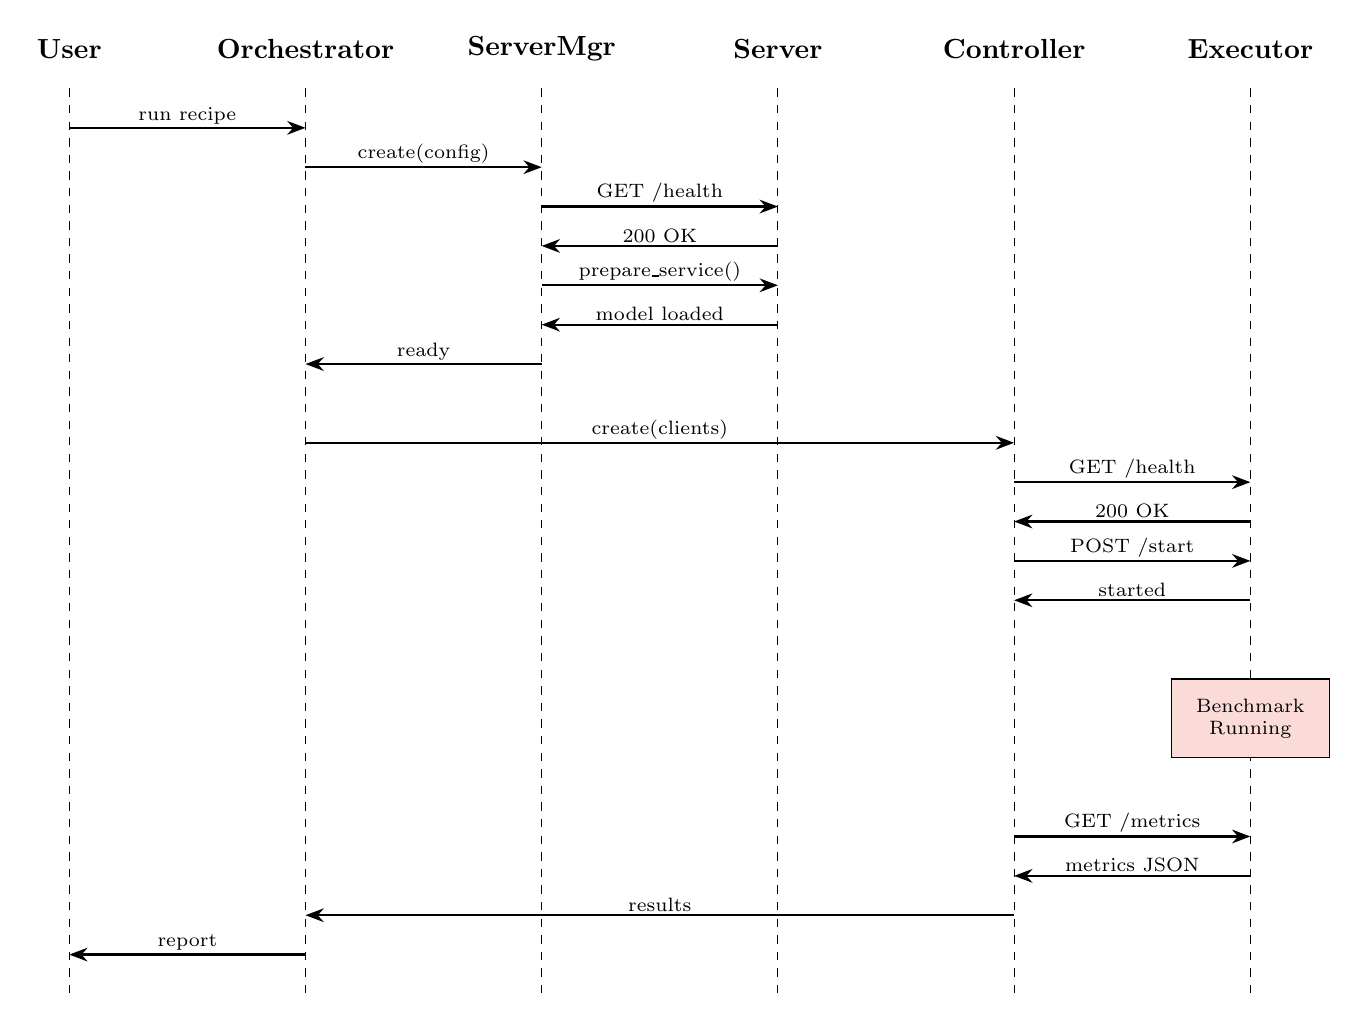
\begin{tikzpicture}[node distance=0.5cm]
    % Participants
    \node (user) at (0, 0) {\textbf{User}};
    \node (orch) at (3, 0) {\textbf{Orchestrator}};
    \node (sm) at (6, 0) {\textbf{ServerMgr}};
    \node (server) at (9, 0) {\textbf{Server}};
    \node (wc) at (12, 0) {\textbf{Controller}};
    \node (exec) at (15, 0) {\textbf{Executor}};

    % Lifelines
    \draw[dashed] (0, -0.5) -- (0, -12);
    \draw[dashed] (3, -0.5) -- (3, -12);
    \draw[dashed] (6, -0.5) -- (6, -12);
    \draw[dashed] (9, -0.5) -- (9, -12);
    \draw[dashed] (12, -0.5) -- (12, -12);
    \draw[dashed] (15, -0.5) -- (15, -12);

    % Messages
    \draw[arrow] (0, -1) -- node[above, font=\scriptsize, fill=white, inner sep=1pt] {run recipe} (3, -1);
    \draw[arrow] (3, -1.5) -- node[above, font=\scriptsize, fill=white, inner sep=1pt] {create(config)} (6, -1.5);
    \draw[arrow] (6, -2) -- node[above, font=\scriptsize, fill=white, inner sep=1pt] {GET /health} (9, -2);
    \draw[arrow] (9, -2.5) -- node[above, font=\scriptsize, fill=white, inner sep=1pt] {200 OK} (6, -2.5);
    \draw[arrow] (6, -3) -- node[above, font=\scriptsize, fill=white, inner sep=1pt] {prepare\_service()} (9, -3);
    \draw[arrow] (9, -3.5) -- node[above, font=\scriptsize, fill=white, inner sep=1pt] {model loaded} (6, -3.5);
    \draw[arrow] (6, -4) -- node[above, font=\scriptsize, fill=white, inner sep=1pt] {ready} (3, -4);

    \draw[arrow] (3, -5) -- node[above, font=\scriptsize, fill=white, inner sep=1pt] {create(clients)} (12, -5);
    \draw[arrow] (12, -5.5) -- node[above, font=\scriptsize, fill=white, inner sep=1pt] {GET /health} (15, -5.5);
    \draw[arrow] (15, -6) -- node[above, font=\scriptsize, fill=white, inner sep=1pt] {200 OK} (12, -6);
    \draw[arrow] (12, -6.5) -- node[above, font=\scriptsize, fill=white, inner sep=1pt] {POST /start} (15, -6.5);
    \draw[arrow] (15, -7) -- node[above, font=\scriptsize, fill=white, inner sep=1pt] {started} (12, -7);

    % Benchmark execution
    \node[draw, fill=accent!20, minimum width=2cm, minimum height=1cm, font=\scriptsize, align=center] at (15, -8.5) {Benchmark\\Running};

    \draw[arrow] (12, -10) -- node[above, font=\scriptsize, fill=white, inner sep=1pt] {GET /metrics} (15, -10);
    \draw[arrow] (15, -10.5) -- node[above, font=\scriptsize, fill=white, inner sep=1pt] {metrics JSON} (12, -10.5);
    \draw[arrow] (12, -11) -- node[above, font=\scriptsize, fill=white, inner sep=1pt] {results} (3, -11);
    \draw[arrow] (3, -11.5) -- node[above, font=\scriptsize, fill=white, inner sep=1pt] {report} (0, -11.5);
\end{tikzpicture}
\caption{Message sequence for benchmark execution}
\end{figure}

% ============================================================================
\section{Execution Flow}
% ============================================================================

\subsection{Seven-Phase Execution Model}

The benchmark execution follows a structured seven-phase model:

\begin{figure}[H]
\centering
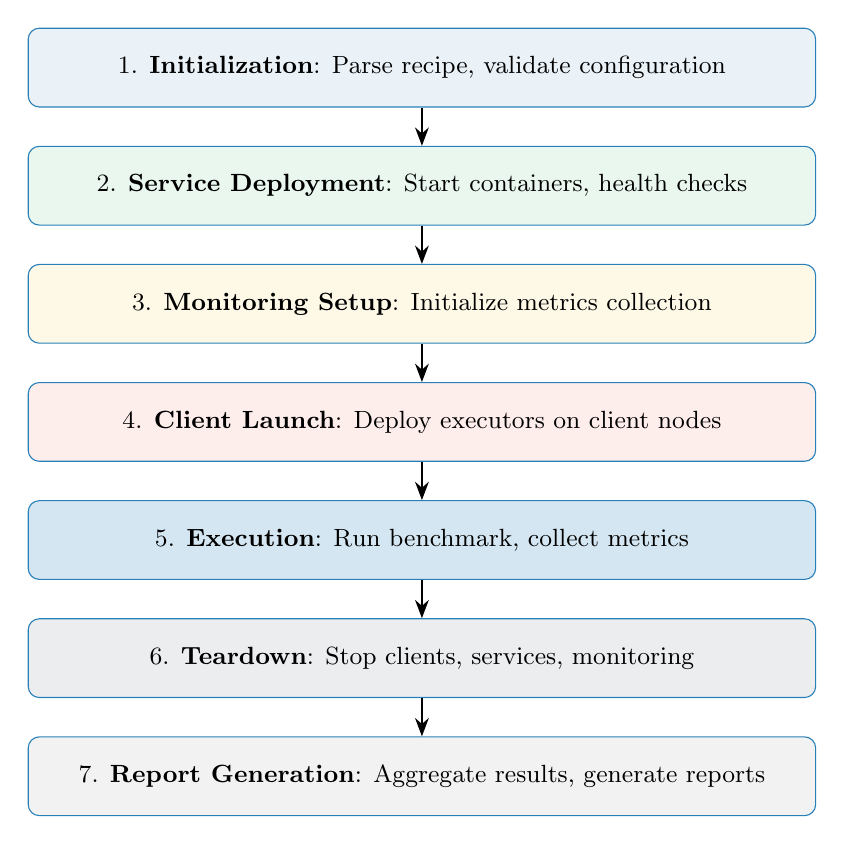
\begin{tikzpicture}[node distance=0.8cm]
    % Phases
    \node[component, minimum width=10cm, fill=primary!10] (p1) at (0, 6) {1. \textbf{Initialization}: Parse recipe, validate configuration};
    \node[component, minimum width=10cm, fill=success!10] (p2) at (0, 4.5) {2. \textbf{Service Deployment}: Start containers, health checks};
    \node[component, minimum width=10cm, fill=warning!10] (p3) at (0, 3) {3. \textbf{Monitoring Setup}: Initialize metrics collection};
    \node[component, minimum width=10cm, fill=accent!10] (p4) at (0, 1.5) {4. \textbf{Client Launch}: Deploy executors on client nodes};
    \node[component, minimum width=10cm, fill=primary!20] (p5) at (0, 0) {5. \textbf{Execution}: Run benchmark, collect metrics};
    \node[component, minimum width=10cm, fill=secondary!10] (p6) at (0, -1.5) {6. \textbf{Teardown}: Stop clients, services, monitoring};
    \node[component, minimum width=10cm, fill=gray!10] (p7) at (0, -3) {7. \textbf{Report Generation}: Aggregate results, generate reports};

    % Arrows
    \draw[arrow] (p1) -- (p2);
    \draw[arrow] (p2) -- (p3);
    \draw[arrow] (p3) -- (p4);
    \draw[arrow] (p4) -- (p5);
    \draw[arrow] (p5) -- (p6);
    \draw[arrow] (p6) -- (p7);
\end{tikzpicture}
\caption{Seven-phase execution model}
\end{figure}

\subsection{Detailed Phase Descriptions}

\subsubsection{Phase 1: Initialization}

\begin{enumerate}
    \item Load and parse YAML recipe file
    \item Validate against JSON schema (\texttt{schemas/recipe-format.yaml})
    \item Expand parameter sweeps (Cartesian product)
    \item Initialize logging and output directories
\end{enumerate}

\subsubsection{Phase 2: Service Deployment}

\begin{enumerate}
    \item Create ServerManager via ServiceFactory
    \item Build endpoint list from server node hostnames
    \item Poll health check endpoints with configurable timeout
    \item Execute service preparation (model loading)
\end{enumerate}

\subsubsection{Phase 3: Monitoring Setup}

This phase sets up the system to track what's happening during the benchmark. It prepares both the HPC cluster and personal laptop to collect performance data:

\begin{enumerate}
    \item \textbf{Start Monitoring}: Turn on the monitor tool that will watch CPU, GPU, and memory usage
    \item \textbf{Choose What to Track}: Decide which metrics to collect (CPU usage, GPU usage, memory, etc.)
    \item \textbf{Connect to Pushgateway}: Set up connection to Prometheus Pushgateway (stores the data)
    \item \textbf{Create Folders}: Make directories to save the collected data as CSV files
    \item \textbf{Run Monitor in Background}: Start monitoring that runs continuously and takes a measurement every 1 second by default
    \item \textbf{Check Grafana Dashboard}: Make sure the dashboard on your laptop is ready to see the data
\end{enumerate}

\textbf{Main Settings:}
\begin{itemize}
    \item \texttt{monitor\_interval}: How often to check the system (example: every 1 second)
    \item \texttt{prometheus\_push\_interval}: How often to send data to storage (example: every 15 seconds)
    \item \texttt{pushgateway\_url}: Where to send the data (example: \texttt{http://mel2109:9091})
    \item \texttt{output\_file}: File name to save results (example: \texttt{benchmark\_metrics.csv})
\end{itemize}

\textbf{Parts of the Monitoring System:}
\begin{itemize}
    \item \textbf{Prometheus on Your Laptop} (port 9092): Collects data every 15 seconds from the HPC cluster
    \item \textbf{Grafana on Your Laptop} (port 3001): Shows graphs and charts of the performance data
    \item \textbf{Pushgateway on HPC}: A storage box that receives metrics from the cluster
    \item \textbf{SSH Tunnels}: Secret paths that let your laptop see the HPC metrics safely
\end{itemize}

\subsubsection{Phase 4: Client Launch}

\begin{enumerate}
    \item Create WorkloadController via ServiceFactory
    \item Verify executor health on all client nodes
    \item Distribute workload configuration
    \item Initialize thread pools on each executor
\end{enumerate}

\subsubsection{Phase 5: Execution}

\begin{enumerate}
    \item Warmup period (configurable duration)
    \item Main benchmark execution
    \item Continuous metrics collection
    \item Real-time Prometheus scraping
\end{enumerate}

\subsubsection{Phase 6: Teardown}

\begin{enumerate}
    \item Send stop signals to all executors
    \item Collect final metrics
    \item Stop monitoring processes
    \item Clean up resources
\end{enumerate}

\subsubsection{Phase 7: Report Generation}

\begin{enumerate}
    \item Aggregate metrics from all clients
    \item Calculate statistics (mean, p50, p90, p99)
    \item Generate CSV/JSON output files
    \item Create summary report
\end{enumerate}

% ============================================================================
\section{Recipe Configuration System}
% ============================================================================

\subsection{Recipe Structure}

Recipes are YAML files that declaratively define benchmark configurations:

\begin{lstlisting}[style=yaml, caption={Complete recipe structure}]
scenario: "experiment-name"
partition: "gpu"
account: "p200981"
qos: "default"

orchestration:
  mode: "slurm"
  total_nodes: 5
  node_allocation:
    servers:
      nodes: 2
    clients:
      nodes: 2
      clients_per_node: 10
    monitors:
      nodes: 1
  job_config:
    time_limit: "02:00:00"
    exclusive: true

resources:
  servers:
    gpus: 2
    cpus_per_task: 1
    mem_gb: 32
  clients:
    gpus: 0
    cpus_per_task: 2
    mem_gb: 16

workload:
  component: "inference"
  service: "ollama"
  duration: "2m"
  warmup: "1m"
  model: "llama2"
  clients_per_node: 10

servers:
  health_check:
    enabled: true
    timeout: 300
    interval: 5
    endpoint: "/api/tags"
  service_config:
    gpu_layers: 0

artifacts:
  containers_dir: "/path/to/containers/"
  service:
    path: "ollama_latest.sif"
  python:
    path: "python_3_12_3_v2.sif"

binds:
  - "/project/.ollama:/root/.ollama:rw"
  - "/project/scratch:/scratch:rw"
\end{lstlisting}

\subsection{Recipe Validation}

\subsection{Recipe Validation System}

To ensure correctness, reproducibility, and safe execution of large-scale benchmarks, the framework implements a comprehensive recipe validation system. Before any Slurm job is generated or submitted, the user-provided YAML recipe is validated both structurally and semantically.

\paragraph{JSON Schema Validation}
At the core of the validation system is a JSON Schema definition that formally specifies the expected structure of a benchmark recipe. The schema enforces required fields, data types, value ranges, and allowed enumerations for all configuration sections, including orchestration, resource allocation, workload parameters, monitoring, and logging. This guarantees that recipes are complete, well-typed, and structurally consistent before execution.

\paragraph{Validation Rules and Error Reporting}
Validation distinguishes between \emph{blocking errors} and \emph{warnings}. Blocking errors correspond to invalid or incomplete configurations that would lead to incorrect execution, such as missing mandatory fields, incompatible service selections, or invalid resource specifications. In these cases, execution is halted. Warnings are issued for configurations that are technically valid but potentially suboptimal, such as unusually high client counts, short benchmark durations, or atypical resource allocations. All validation messages are reported with clear, field-level context to facilitate rapid correction by the user.

\paragraph{Custom Validators}
In addition to schema-based checks, the system implements custom validation logic to capture constraints that cannot be expressed declaratively. These include cross-field consistency checks, service-specific requirements, and semantic constraints, such as verifying that inference workloads specify the necessary model and prompt parameters, or that node allocations are consistent with the declared total number of nodes.

\paragraph{Schema Versioning}
To support long-term maintainability and reproducibility, the validation system includes schema versioning. This allows recipes to be validated against a specific schema version, ensuring that experiments remain reproducible even as the configuration format evolves over time. Backward compatibility can be maintained while enabling controlled extensions of the recipe format.

\paragraph{Interactive Validation Mode}
The framework provides an interactive validation mode that allows users to validate recipes locally before submission. This enables early detection of configuration issues without consuming HPC resources and improves usability by providing immediate feedback during experiment design.

Overall, the recipe validation system plays a crucial role in preventing invalid job submissions, reducing wasted computational resources, and ensuring consistent and reproducible benchmarking experiments.

\subsection{Parameter Sweeps}

The recipe system supports automatic parameter expansion:

\begin{lstlisting}[style=yaml, caption={Parameter sweep configuration}]
workload:
  batch: [1, 4, 8]           # 3 values
  concurrency: [1, 8, 32]    # 3 values
  prompt_len: [128, 512]     # 2 values
  # Total trials: 3 x 3 x 2 = 18
\end{lstlisting}

% ============================================================================
\section{Distributed Benchmarking with Ray}
% ============================================================================

\subsection{Ray Cluster Architecture}

For distributed vLLM deployments, the toolkit integrates with Ray for tensor and pipeline parallelism:

\begin{figure}[H]
\centering
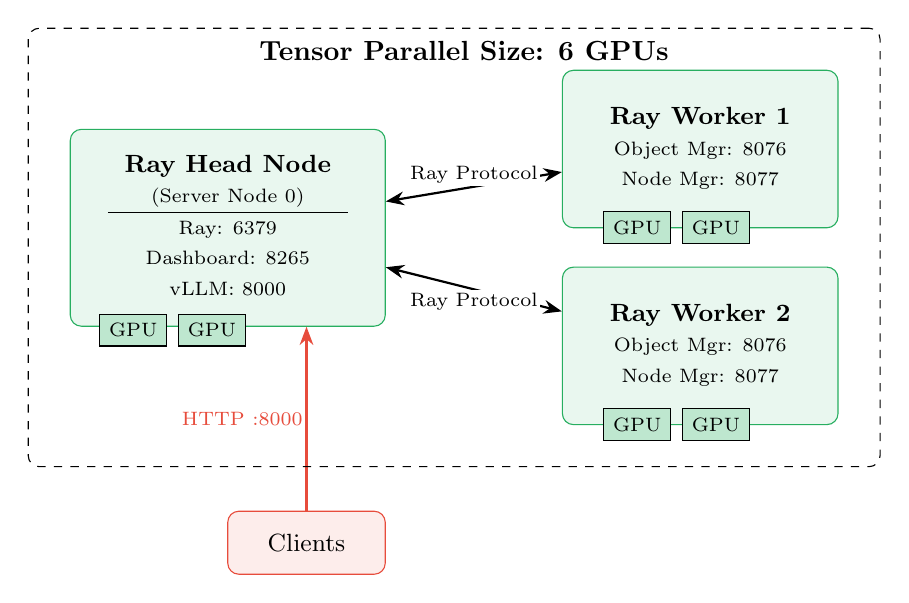
\begin{tikzpicture}[node distance=1.5cm]
    % Ray Head Node
    \node[server, minimum width=4cm, minimum height=2.5cm] (head) at (-3, 0) {
        \begin{tabular}{c}
            \textbf{Ray Head Node} \\
            \scriptsize (Server Node 0) \\
            \hline
            \scriptsize Ray: 6379 \\
            \scriptsize Dashboard: 8265 \\
            \scriptsize vLLM: 8000
        \end{tabular}
    };

    % Ray Worker Nodes
    \node[server, minimum width=3.5cm, minimum height=2cm] (w1) at (3, 1) {
        \begin{tabular}{c}
            \textbf{Ray Worker 1} \\
            \scriptsize Object Mgr: 8076 \\
            \scriptsize Node Mgr: 8077
        \end{tabular}
    };

    \node[server, minimum width=3.5cm, minimum height=2cm] (w2) at (3, -1.5) {
        \begin{tabular}{c}
            \textbf{Ray Worker 2} \\
            \scriptsize Object Mgr: 8076 \\
            \scriptsize Node Mgr: 8077
        \end{tabular}
    };

    % GPU icons
    \node[draw, fill=success!30, minimum width=0.8cm, font=\scriptsize] at (-4.2, -1.3) {GPU};
    \node[draw, fill=success!30, minimum width=0.8cm, font=\scriptsize] at (-3.2, -1.3) {GPU};
    \node[draw, fill=success!30, minimum width=0.8cm, font=\scriptsize] at (2.2, 0) {GPU};
    \node[draw, fill=success!30, minimum width=0.8cm, font=\scriptsize] at (3.2, 0) {GPU};
    \node[draw, fill=success!30, minimum width=0.8cm, font=\scriptsize] at (2.2, -2.5) {GPU};
    \node[draw, fill=success!30, minimum width=0.8cm, font=\scriptsize] at (3.2, -2.5) {GPU};

    % Connections
    \draw[biarrow, thick] (head) -- node[above, font=\scriptsize, fill=white, inner sep=1pt] {Ray Protocol} (w1);
    \draw[biarrow, thick] (head) -- node[below, font=\scriptsize, fill=white, inner sep=1pt] {Ray Protocol} (w2);

    % Client requests
    \node[client, minimum width=2cm] (client) at (-2, -4) {Clients};
    \draw[arrow, accent] (client) -- node[left, font=\scriptsize, fill=white, inner sep=1pt] {HTTP :8000 } ([xshift=1cm]head.south);

    % Tensor parallelism label
    \node[draw, dashed, rounded corners, fit=(head)(w1)(w2), inner sep=15pt] {};
    \node[above] at (0, 2) {\textbf{Tensor Parallel Size: 6 GPUs}};
\end{tikzpicture}
\caption{Ray cluster architecture for distributed vLLM}
\end{figure}

\subsection{RayClusterManager}

The \texttt{RayClusterManager} class handles Ray cluster lifecycle:

\begin{lstlisting}[style=python, caption={RayClusterManager key methods}]
class RayClusterManager:
    def start_head_node(self, port: int = 6379) -> bool:
        """Initialize Ray head node with ray start --head"""
        cmd = f"ray start --head --port={port}"
        # Execute and verify

    def connect_worker(self, head_address: str) -> bool:
        """Connect worker to existing Ray cluster"""
        cmd = f"ray start --address={head_address}"
        # Execute and verify

    def get_head_ip(self) -> str:
        """Auto-detect local IP for Ray communication"""
        # Network interface detection
\end{lstlisting}

\subsection{Distributed vLLM Configuration}

\begin{lstlisting}[style=yaml, caption={Distributed vLLM recipe configuration}]
servers:
  service_config:
    distributed:
      enabled: true
      backend: "ray"
      tensor_parallel_size: 4
      pipeline_parallel_size: 1
      ray:
        dashboard_port: 8265
        object_manager_port: 8076
        node_manager_port: 8077
        num_cpus_per_node: 4
        num_gpus_per_node: 2
    max_model_len: 2048
    gpu_memory_utilization: 0.7
\end{lstlisting}

% ============================================================================
\section{Monitoring System}
% ============================================================================

The monitoring system watches what happens during the benchmark and shows you the results. It has two main parts: one on the HPC cluster that collects data, and one on your laptop that shows graphs of this data.

\subsection{How Monitoring Works}

\textbf{Simple Overview:}

\begin{enumerate}
    \item Client computers on HPC measure CPU, GPU, and memory usage every second
    \item These measurements are stored and sent to a storage server
    \item Your laptop connects to the HPC cluster through a secure tunnel
    \item Your laptop collects these measurements every 15 seconds
    \item Your laptop shows you graphs of all this data in Grafana
\end{enumerate}

\subsection{Data Collection on HPC}

\begin{figure}[H]
\centering
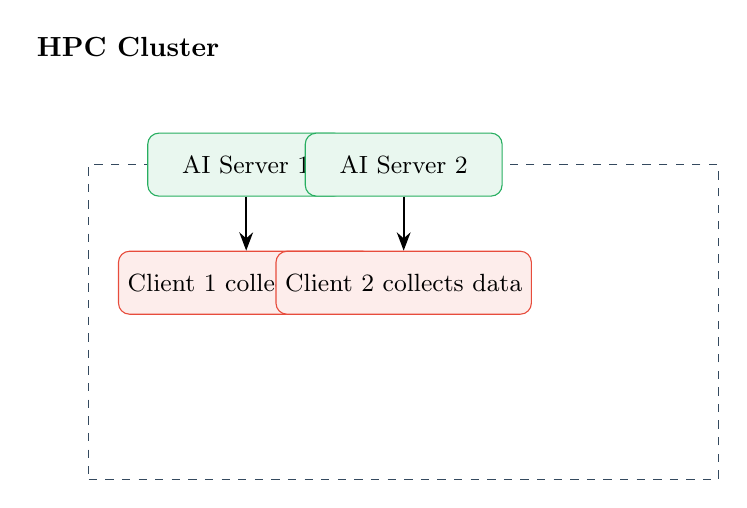
\begin{tikzpicture}[node distance=1.2cm]
    % HPC Cluster
    \node[container, minimum width=8cm, minimum height=4cm] (hpc) at (0, 0) {};
    \node at (-3.5, 3.5) {\textbf{HPC Cluster}};
    
    % Server nodes
    \node[server] (srv1) at (-2, 2) {AI Server 1};
    \node[server] (srv2) at (0, 2) {AI Server 2};
    
    % Client nodes with executors
    \node[client] (cli1) at (-2, 0.5) {Client 1 collects data};
    \node[client] (cli2) at (0, 0.5) {Client 2 collects data};
    
    % Connections
    \draw[arrow] (srv1) -- (cli1);
    \draw[arrow] (srv2) -- (cli2);
\end{tikzpicture}
\end{figure}

On the HPC cluster, each client computer has a small Python program that:
\begin{enumerate}
    \item Measures system performance (CPU, GPU, memory) every 1 second
    \item Stores these measurements in memory
    \item Provides them through a web endpoint on port 6000
\end{enumerate}

\subsection{Data Viewing on Your Laptop}

\begin{figure}[H]
\centering
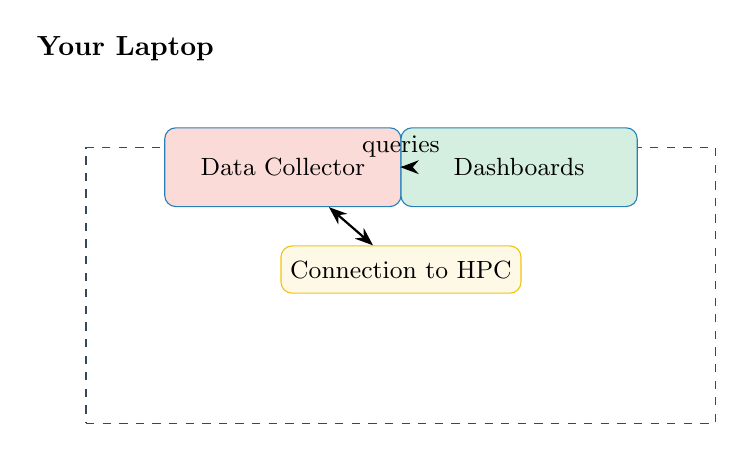
\begin{tikzpicture}[node distance=1.2cm]
    % Laptop
    \node[container, minimum width=8cm, minimum height=3.5cm] (laptop) at (0, 0) {};
    \node at (-3.5, 3) {\textbf{Your Laptop}};
    
    % Prometheus
    \node[component, fill=accent!20] (prom) at (-1.5, 1.5) {Data Collector};
    
    % Grafana
    \node[component, fill=success!20] (graf) at (1.5, 1.5) {Dashboards};
    
    % Tunnel
    \node[monitor, minimum height=0.6cm] (tunnel) at (0, 0.2) {Connection to HPC};
    
    % Connections
    \draw[biarrow] (prom) -- (tunnel);
    \draw[arrow] (prom) -- (graf) node[above, midway, font=\small] {queries};
\end{tikzpicture}
\end{figure}

On the laptop, there are two programs:

\begin{enumerate}
    \item \textbf{Prometheus} (on port 9092): A program that collects data from HPC every 15 seconds through the secure tunnel
    \item \textbf{Grafana} (on port 3001): A program that creates nice graphs from the collected data
\end{enumerate}

\subsection{Step-by-Step: From HPC to Your Dashboard}

\textbf{Step 1: HPC Client Collects Data}

On client computers on HPC, a Python monitor continuously runs:

\begin{lstlisting}[style=bash]
# Data is available here on HPC (inside the cluster)
http://client-node:6000/metrics/prometheus

# The data looks like:
ollama_throughput_rps 578           # 578 requests per second
ollama_workload_running 1           # 1 = workload is running
ollama_request_latency_seconds 0.015  # Each request takes 15ms
\end{lstlisting}

\textbf{Step 2: Create a Tunnel to HPC}

Since your laptop cannot directly see HPC, a secure tunnel is created:

\begin{lstlisting}[style=bash]
# Example: Create tunnel from your port 25000 to HPC client-node port 6000
ssh -N -L 25000:client-node:6000 meluxina &

# Now you can see HPC data from your laptop at:
http://localhost:25000/metrics/prometheus
\end{lstlisting}

\textbf{Step 3: Prometheus Reads the Data}

A program called Prometheus on your laptop reads from this tunnel:

\begin{lstlisting}[style=bash]
# Prometheus configuration file tells it where to look
# It checks every 15 seconds
scrape_configs:
  - job_name: 'ollama'
    static_configs:
      - targets: ['localhost:25000', 'localhost:25001']
\end{lstlisting}

\textbf{Step 4: Grafana Shows You the Graphs}

Grafana reads the stored data from Prometheus and shows nice graphs:

\begin{itemize}
    \item A number showing if the workload is running (0 means stopped, 1 means running)
    \item A line graph showing requests per second over time
    \item A line graph showing response time over time
    \item Counters showing total successes and failures
\end{itemize}

\subsection{What the Dashboards Show}

\textbf{Ollama Performance Dashboard}

This shows performance of the Ollama AI model:

\begin{itemize}
    \item \textbf{Is it Running?}: Shows 0 (stopped) or 1 (running)
    \item \textbf{Total Requests}: How many AI requests have been made (goes up over time)
    \item \textbf{Speed per Computer}: Shows requests/sec on each computer (line graph)
    \item \textbf{Total Speed}: Shows all requests/sec combined (big number)
    \item \textbf{Response Time}: How long each request takes (line graph in milliseconds)
    \item \textbf{Success vs Failure}: Comparison of successful vs failed requests (bar chart)
    \item \textbf{Error Percentage}: What percent of requests failed (line graph)
\end{itemize}

\textbf{vLLM Performance Dashboard}

Same metrics of the Ollama but for the vLLM AI model, with extra panels:

\begin{itemize}
    \item \textbf{Tokens per Request}: How many words the AI generates per request
    \item \textbf{Cache Usage}: How full the GPU cache is (as a percentage)
\end{itemize}

\subsection{SSH Tunneling for Metrics}
\begin{itemize}
    \item \textbf{Ollama Dashboard}: 13 panels monitoring Ollama workload metrics
    \begin{itemize}
        \item Workload Status (gauge: 0=idle, 1=running)
        \item Requests Total (counter)
        \item Throughput by Host (timeseries)
        \item Total Throughput (stat panel in RPS)
        \item Request Latency (timeseries in ms)
        \item Success vs Failed Requests (bar chart)
        \item Error Rate Over Time (percentage)
        \item Plus additional CPU/GPU/Memory panels
    \end{itemize}
    
    \item \textbf{vLLM Dashboard}: Same layout with vLLM-specific metrics
    \begin{itemize}
        \item vllm\_workload\_running
        \item vllm\_throughput\_rps
        \item vllm\_request\_latency\_seconds
        \item vllm\_tokens\_per\_request
        \item vllm\_cache\_usage
    \end{itemize}
\end{itemize}

\textbf{Example Grafana Queries:}
\begin{lstlisting}[style=bash]
# Current workload status
ollama_workload_running

# Throughput aggregated across hosts
sum(ollama_throughput_rps)

# Latency p95
histogram_quantile(0.95, ollama_request_latency_seconds)

# Error rate
100 * (sum(rate(ollama_errors_total[5m])) / sum(rate(ollama_requests_total[5m])))
\end{lstlisting}

\subsection{SSH Tunneling for Metrics Access}

\begin{enumerate}
    \item \textbf{Find client nodes from job output}:
    \begin{lstlisting}[style=bash]
ssh meluxina "scontrol show job JOBID | grep StdOut"
ssh meluxina "cat /path/to/logs/*.out" | grep "Client nodes"
    \end{lstlisting}
    
    \item \textbf{Open SSH tunnels}:
    \begin{lstlisting}[style=bash]
# Ollama clients
ssh -N -L 25000:mel2120:6000 meluxina &
ssh -N -L 25001:mel2148:6000 meluxina &

# vLLM clients
ssh -N -L 25002:mel2142:6000 meluxina &
ssh -N -L 25003:mel2185:6000 meluxina &
    \end{lstlisting}
    
    \item \textbf{Verify metrics endpoint}:
    \begin{lstlisting}[style=bash]
curl http://localhost:25000/metrics/prometheus | head -5
    \end{lstlisting}
    
    \item \textbf{Access Grafana}:
    \begin{lstlisting}[style=bash]
open http://localhost:3001  # admin / admin
    \end{lstlisting}
\end{enumerate}

% ============================================================================
\section{Benchmarking Implementation}
% ============================================================================

\section{Benchmarking System}

This section documents the implementation of the benchmarking subsystem, focusing exclusively on how inference workloads are generated, executed, and measured. The benchmarking logic is implemented at the client side through workload executors and is coordinated by the orchestrator.

\subsection{Workload Executor Implementation}

The workload executor is responsible for generating load against inference services and collecting performance metrics. Each executor runs on a client node and exposes an HTTP interface for control and metric retrieval.

\paragraph{Thread Pool Management}
Concurrency is implemented using a thread-based execution model. Upon receiving a start command, the executor spawns a configurable number of worker threads (\texttt{num\_threads}), each of which independently generates requests. Threads run concurrently for the specified benchmark duration and terminate gracefully once execution completes.

\paragraph{Request Generation}
Each worker thread repeatedly issues inference requests to the configured service endpoints until the benchmark duration expires. Requests are distributed across available server endpoints using a round-robin strategy to balance load. An optional inter-request delay (\texttt{sleep\_seconds}) allows precise control over request pacing, enabling both latency-focused and throughput-focused benchmarks.

\paragraph{Latency Measurement}
Latency is measured on a per-request basis as the elapsed wall-clock time between request submission and response reception. Each thread records individual request latencies locally, enabling detailed latency distribution analysis after execution.

\paragraph{Error Handling}
All request execution is wrapped in exception handling logic. HTTP failures and runtime exceptions are counted as errors and recorded without terminating the benchmark. This ensures that transient failures or service overload conditions are reflected accurately in the collected metrics.

\subsection{Ollama Benchmarking}

Ollama benchmarking is implemented via a service-specific workload executor targeting the Ollama HTTP inference API.

\paragraph{HellaSwag Dataset Integration}
To generate realistic inference prompts, the executor integrates the HellaSwag validation dataset. The dataset is loaded once per executor instance and shared across worker threads. Each request samples a random prompt from the dataset, ensuring diversity and avoiding synthetic prompt bias.

\paragraph{Request Format}
Inference requests are sent to the Ollama \texttt{/api/generate} endpoint using non-streaming mode. Each request specifies the target model and the selected prompt text. Streaming responses are disabled to ensure clear request boundaries and consistent latency measurement.

\paragraph{Response Handling}
Responses are validated based on HTTP status codes. Successful responses contribute to latency and throughput metrics, while failed responses increment error counters. Response payloads are not parsed further, as token-level usage information is not consistently exposed by the Ollama API.

\paragraph{Metrics Collection}
Each worker thread reports the total number of requests, error count, cumulative latency, elapsed execution time, and a list of per-request latencies. These thread-level metrics are aggregated at the executor level after benchmark completion.

\subsection{vLLM Benchmarking}

The benchmarking framework supports vLLM-based inference via its OpenAI-compatible API. In this implementation, benchmarking focuses on non-streaming request execution. While the system supports both single-node and distributed vLLM deployments, streaming behavior and detailed token accounting are not benchmarked in this work.

\subsection{Metrics Collection}

Metrics are collected hierarchically, starting at the per-request level and aggregated across threads and executors.

\paragraph{Latency Percentiles}
In addition to average latency, the system computes latency percentiles (p50, p90, p99) from all recorded request latencies. These metrics capture tail latency behavior, which is critical for evaluating inference performance under concurrent load.

\paragraph{Throughput}
Throughput is calculated as the total number of successful requests divided by the maximum elapsed execution time across threads. This provides a conservative estimate of sustained request processing capacity.

\paragraph{Error Rates}
Error rates are computed as the ratio of failed requests to total requests. This metric highlights service instability or overload conditions during benchmarking.

\paragraph{Resource Utilization}
While resource utilization metrics are collected externally via the monitoring subsystem, the benchmarking layer exposes timing and request-level metrics that can be correlated with system-level resource data.

\subsection{Load Patterns}

The implemented benchmarking system generates constant load with configurable concurrency and request pacing. While the framework design allows for more complex load patterns such as Poisson or bursty arrivals, these patterns are not implemented in the current version and are reserved for future work.

% ============================================================================
\section{Logging System}
% ============================================================================

\subsection{Overview}

The logging system provides comprehensive log aggregation and management across distributed HPC benchmark executions. It collects, aggregates, and stores logs from multiple nodes in a centralized, structured format suitable for analysis and debugging.

\subsubsection{Design Goals}

The logging system was designed with the following objectives:

\begin{itemize}
    \item \textbf{Multi-Node Aggregation}: Collect logs from distributed server and client nodes into centralized files
    \item \textbf{Structured Output}: Provide both human-readable and machine-parseable (JSON) log formats
    \item \textbf{Extensibility}: Support multiple log collection implementations through abstract interfaces
    \item \textbf{Real-Time Collection}: Capture logs continuously during benchmark execution
    \item \textbf{Minimal Overhead}: Use lightweight file tailing to avoid performance impact
\end{itemize}

\subsection{Architecture}

The logging system employs the Strategy pattern to provide a flexible, extensible architecture. Figure~\ref{fig:logging-architecture} illustrates the high-level architecture.

\begin{figure}[H]
\centering
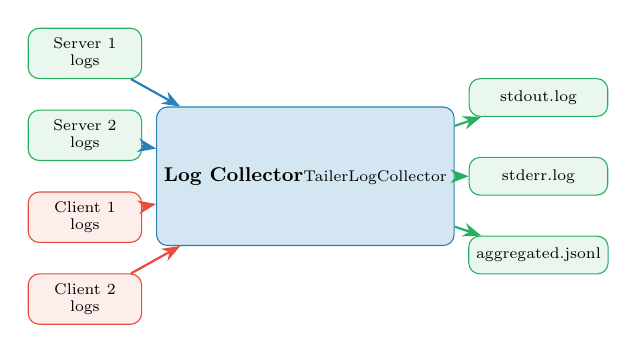
\begin{tikzpicture}[node distance=1cm, scale=0.8, every node/.style={scale=0.8}]
    % Distributed sources
    \node[server, minimum width=1.8cm, font=\scriptsize] (s1) at (-3, 2.5) {\shortstack{Server 1\\logs}};
    \node[server, minimum width=1.8cm, font=\scriptsize] (s2) at (-3, 1.2) {\shortstack{Server 2\\logs}};
    \node[client, minimum width=1.8cm, font=\scriptsize] (c1) at (-3, -0.1) {\shortstack{Client 1\\logs}};
    \node[client, minimum width=1.8cm, font=\scriptsize] (c2) at (-3, -1.4) {\shortstack{Client 2\\logs}};
    
    % Log Collector
    \node[component, minimum width=3cm, minimum height=2.2cm, fill=primary!20] (collector) at (0.5, 0.55) {
        \textbf{Log Collector}\par
        {\scriptsize TailerLogCollector}
    };
    
    % Aggregated outputs
    \node[component, minimum width=2.2cm, minimum height=0.6cm, font=\scriptsize, fill=success!10, draw=success] (out1) at (4.2, 1.8) {stdout.log};
    \node[component, minimum width=2.2cm, minimum height=0.6cm, font=\scriptsize, fill=success!10, draw=success] (out2) at (4.2, 0.55) {stderr.log};
    \node[component, minimum width=2.2cm, minimum height=0.6cm, font=\scriptsize, fill=success!10, draw=success] (out3) at (4.2, -0.7) {aggregated.jsonl};
    
    % Arrows
    \draw[arrow, primary] (s1) -- (collector);
    \draw[arrow, primary] (s2) -- (collector);
    \draw[arrow, accent] (c1) -- (collector);
    \draw[arrow, accent] (c2) -- (collector);
    \draw[arrow, success] (collector) -- (out1);
    \draw[arrow, success] (collector) -- (out2);
    \draw[arrow, success] (collector) -- (out3);
\end{tikzpicture}
\caption{Logging system architecture}
\label{fig:logging-architecture}
\end{figure}

\subsubsection{Strategy Pattern Implementation}

The logging system uses the Strategy pattern to allow different log collection implementations while maintaining a consistent interface. Figure~\ref{fig:logging-strategy} shows the class hierarchy.

\begin{figure}[H]
\centering
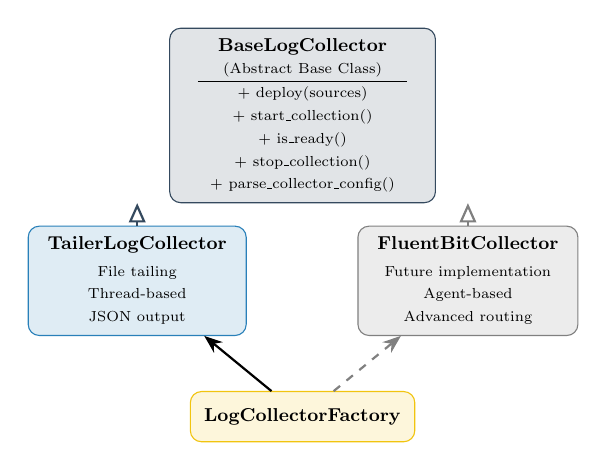
\begin{tikzpicture}[node distance=1.5cm, scale=0.75, every node/.style={scale=0.75}]
    % Abstract base
    \node[component, minimum width=4.5cm, minimum height=2.3cm, fill=secondary!15, draw=secondary] (base) at (0, 2.8) {
        \begin{tabular}{c}
            \textbf{BaseLogCollector}\\
            {\scriptsize (Abstract Base Class)}\\
            \hline
            {\scriptsize + deploy(sources)}\\
            {\scriptsize + start\_collection()}\\
            {\scriptsize + is\_ready()}\\
            {\scriptsize + stop\_collection()}\\
            {\scriptsize + parse\_collector\_config()}
        \end{tabular}
    };
    
    % Concrete implementations
    \node[component, minimum width=3.5cm, minimum height=1.6cm, fill=primary!15] (tailer) at (-2.8, 0) {
        \begin{tabular}{c}
            \textbf{TailerLogCollector}\\[2pt]
            {\scriptsize File tailing}\\
            {\scriptsize Thread-based}\\
            {\scriptsize JSON output}
        \end{tabular}
    };
    
    \node[component, minimum width=3.5cm, minimum height=1.6cm, fill=gray!15, draw=gray] (future) at (2.8, 0) {
        \begin{tabular}{c}
            \textbf{FluentBitCollector}\\[2pt]
            {\scriptsize Future implementation}\\
            {\scriptsize Agent-based}\\
            {\scriptsize Advanced routing}
        \end{tabular}
    };
    
    % Factory
    \node[component, minimum width=3.8cm, minimum height=0.85cm, fill=warning!15, draw=warning, font=\small] (factory) at (0, -2.3) {
        \textbf{LogCollectorFactory}
    };
    
    % Inheritance arrows
    \draw[thick, -{Triangle[open, length=7pt, width=6pt]}, secondary] (tailer.north) -- (base.south -| tailer);
    \draw[thick, -{Triangle[open, length=7pt, width=6pt]}, gray] (future.north) -- (base.south -| future);
    
    % Factory arrows
    \draw[arrow] (factory) -- (tailer);
    \draw[arrow, dashed, gray] (factory) -- (future);
\end{tikzpicture}
\caption{Strategy pattern in logging system}
\label{fig:logging-strategy}
\end{figure}

\subsection{Core Components}

\subsubsection{LogSource Dataclass}

The \texttt{LogSource} dataclass provides a structured representation of a single log source:

\begin{lstlisting}[style=python, caption={LogSource dataclass definition}]
@dataclass
class LogSource:
    """
    Represents a single source of logs to collect.
    
    Attributes:
        node: Node hostname where logs are generated
        component: Type of component ("server", "client", "monitor")
        container_name: Name/ID of the container producing logs
    """
    node: str
    component: str
    container_name: str
\end{lstlisting}

Example usage:

\begin{lstlisting}[style=python, caption={LogSource example}]
# Create a log source for a server node
log_source = LogSource(
    node="mel2120",
    component="server",
    container_name="ollama_0"
)

# Create a log source for a client node
client_source = LogSource(
    node="mel2148",
    component="client",
    container_name="python_executor_1"
)
\end{lstlisting}

\subsubsection{BaseLogCollector Interface}

The \texttt{BaseLogCollector} abstract class defines the interface that all log collector implementations must follow:

\begin{lstlisting}[style=python, caption={BaseLogCollector abstract methods}]
class BaseLogCollector(ABC):
    """Abstract base class for managing log collection operations."""
    
    @abstractmethod
    def deploy(self, sources: List[LogSource]) -> bool:
        """
        Deploy log collection infrastructure.
        
        Args:
            sources: List of log sources to collect from
            
        Returns:
            True if deployment succeeded, False otherwise
        """
        pass
    
    @abstractmethod
    def start_collection(self) -> bool:
        """
        Start collecting logs from all deployed sources.
        
        Returns:
            True if collection started successfully
        """
        pass
    
    @abstractmethod
    def is_ready(self) -> bool:
        """
        Check if log collector is ready to collect logs.
        
        Returns:
            True if ready, False otherwise
        """
        pass
    
    @abstractmethod
    def stop_collection(self) -> Dict[str, Any]:
        """
        Stop log collection and finalize outputs.
        
        Returns:
            Dictionary with collection summary/metadata
        """
        pass
\end{lstlisting}

\subsection{TailerLogCollector Implementation}

The \texttt{TailerLogCollector} provides a lightweight, thread-based implementation that tails log files and aggregates them into centralized outputs.

\subsubsection{Architecture}

The TailerLogCollector operates in five distinct phases:

\begin{enumerate}
    \item \textbf{Deploy Phase}: Create output files (stdout.log, stderr.log, aggregated.jsonl)
    \item \textbf{Start Phase}: Launch one thread per log source, create "loggers\_ready" flag
    \item \textbf{Tail Phase}: Each thread monitors its log file, reading new lines continuously
    \item \textbf{Process Phase}: Add timestamp, node, and component metadata to each log line
    \item \textbf{Stop Phase}: Stop threads, close files, return summary with line counts and file paths
\end{enumerate}

\begin{figure}[H]
\centering
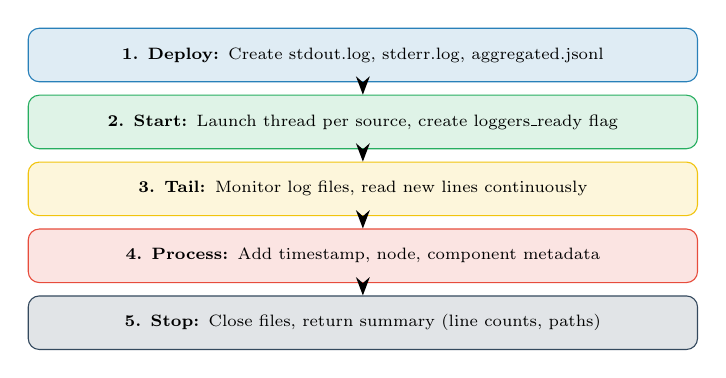
\begin{tikzpicture}[node distance=0.7cm, scale=0.85, every node/.style={scale=0.85}]
    \node[component, minimum width=10cm, minimum height=0.8cm, fill=primary!15, text width=9.5cm, font=\scriptsize] (s1) at (0, 0) {
        \textbf{1. Deploy:} Create stdout.log, stderr.log, aggregated.jsonl
    };
    
    \node[component, minimum width=10cm, minimum height=0.8cm, fill=success!15, draw=success, text width=9.5cm, font=\scriptsize] (s2) at (0, -1) {
        \textbf{2. Start:} Launch thread per source, create loggers\_ready flag
    };
    
    \node[component, minimum width=10cm, minimum height=0.8cm, fill=warning!15, draw=warning, text width=9.5cm, font=\scriptsize] (s3) at (0, -2) {
        \textbf{3. Tail:} Monitor log files, read new lines continuously
    };
    
    \node[component, minimum width=10cm, minimum height=0.8cm, fill=accent!15, draw=accent, text width=9.5cm, font=\scriptsize] (s4) at (0, -3) {
        \textbf{4. Process:} Add timestamp, node, component metadata
    };
    
    \node[component, minimum width=10cm, minimum height=0.8cm, fill=secondary!15, draw=secondary, text width=9.5cm, font=\scriptsize] (s5) at (0, -4) {
        \textbf{5. Stop:} Close files, return summary (line counts, paths)
    };
    
    % Arrows
    \draw[arrow, thick] (s1.south) -- (s2.north);
    \draw[arrow, thick] (s2.south) -- (s3.north);
    \draw[arrow, thick] (s3.south) -- (s4.north);
    \draw[arrow, thick] (s4.south) -- (s5.north);
\end{tikzpicture}
\caption{TailerLogCollector workflow}
\end{figure}

\subsubsection{Configuration}

TailerLogCollector is configured via the recipe YAML file:

\begin{lstlisting}[style=yaml, caption={TailerLogCollector configuration in recipe}]
logging:
  type: "tailer"
  create_jsonl: true
  flush_interval: 5
  
  outputs:
    stdout: "stdout.log"
    stderr: "stderr.log"
    aggregated: "aggregated.jsonl"
\end{lstlisting}

Configuration parameters:

\begin{table}[H]
\centering
\begin{tabular}{@{}llp{8cm}@{}}
\toprule
\textbf{Parameter} & \textbf{Default} & \textbf{Description} \\
\midrule
type & "tailer" & Collector implementation type \\
create\_jsonl & true & Enable structured JSON output \\
flush\_interval & 5 & Buffer flush interval in seconds \\
outputs.stdout & "stdout.log" & Path for stdout aggregation \\
outputs.stderr & "stderr.log" & Path for stderr aggregation \\
outputs.aggregated & "aggregated.jsonl" & Path for JSON Lines output \\
\bottomrule
\end{tabular}
\caption{TailerLogCollector configuration parameters}
\end{table}

\subsubsection{Implementation Details}

\textbf{Thread-Based Tailing:}

\begin{lstlisting}[style=python, caption={Thread-based log tailing implementation}]
def _tail_log_file(self, source: LogSource, log_file: Path):
    """Tail a log file and write to aggregated outputs."""
    print(f"Starting tail for {log_file}")
    
    # Wait for file to exist
    while not log_file.exists() and not self.stop_event.is_set():
        time.sleep(1)
    
    if self.stop_event.is_set():
        return
    
    try:
        with open(log_file, 'r') as f:
            while not self.stop_event.is_set():
                line = f.readline()
                
                if line:
                    self._process_log_line(source, line.rstrip('\n'))
                else:
                    time.sleep(0.1)
                    
    except Exception as e:
        print(f"Error tailing {log_file}: {e}")
\end{lstlisting}

\textbf{Log Line Processing:}

\begin{lstlisting}[style=python, caption={Log line processing with metadata}]
def _process_log_line(self, source: LogSource, line: str):
    """Process a single log line from a source."""
    try:
        timestamp = datetime.utcnow().isoformat() + 'Z'
        
        # Write to aggregated stdout with metadata
        log_entry = f"[{timestamp}] [{source.node}] [{source.component}] {line}\n"
        self.stdout_handle.write(log_entry)
        
        # Write to structured .jsonl
        if self.create_jsonl and self.jsonl_handle:
            jsonl_entry = {
                "timestamp": timestamp,
                "node": source.node,
                "component": source.component,
                "message": line
            }
            self.jsonl_handle.write(json.dumps(jsonl_entry) + '\n')
            
    except Exception as e:
        print(f"Error processing log line: {e}")
\end{lstlisting}

\subsection{Log Output Formats}

The logging system produces three output files, each serving a different purpose:

\subsubsection{stdout.log - Plain Text with Metadata}

Human-readable format with timestamp, node, and component prefixes:

\begin{lstlisting}[style=bash, caption={stdout.log example}]
[2026-01-12T14:32:15Z] [mel2120] [server] Model loaded successfully
[2026-01-12T14:32:16Z] [mel2148] [client] Started 100 worker threads
[2026-01-12T14:32:17Z] [mel2120] [server] Ready to accept connections
[2026-01-12T14:32:18Z] [mel2148] [client] Benchmark warmup phase started
\end{lstlisting}

\subsubsection{stderr.log - Error Messages}

Contains error messages and warnings (typically empty for successful runs):

\begin{lstlisting}[style=bash, caption={stderr.log example}]
[2026-01-12T14:35:20Z] [mel2148] [client] Connection timeout to server
[2026-01-12T14:35:21Z] [mel2148] [client] Retrying connection (attempt 2/3)
\end{lstlisting}

\subsubsection{aggregated.jsonl - Structured JSON Lines}

Machine-parseable format for automated analysis:

\begin{lstlisting}[style=python, caption={aggregated.jsonl example}]
{"timestamp": "2026-01-12T14:32:15Z", "node": "mel2120", "component": "server", "message": "Model loaded successfully"}
{"timestamp": "2026-01-12T14:32:16Z", "node": "mel2148", "component": "client", "message": "Started 100 worker threads"}
{"timestamp": "2026-01-12T14:32:17Z", "node": "mel2120", "component": "server", "message": "Ready to accept connections"}
\end{lstlisting}

\subsection{Multi-Node Log Aggregation}

One of the key challenges in HPC benchmarking is collecting logs from distributed nodes and merging them into a coherent timeline. The logging system achieves this through timestamp-based aggregation.

\subsubsection{Aggregation Strategy}

\begin{figure}[H]
\centering
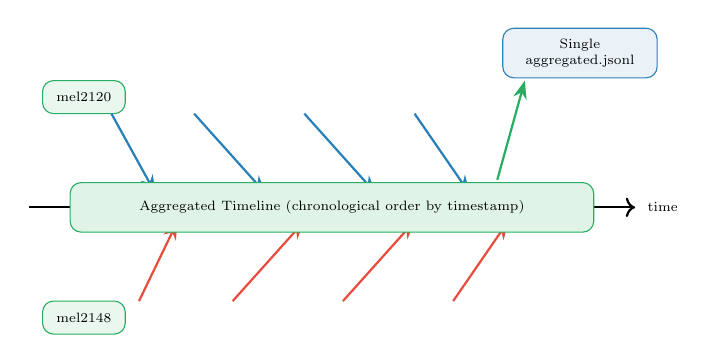
\begin{tikzpicture}[node distance=1cm, scale=0.7, every node/.style={scale=0.7}]
    % Timeline
    \draw[thick, ->] (-5.5, 0) -- (5.5, 0);
    \node at (6, 0) {\scriptsize time};
    
    % Node 1 logs
    \node[server, minimum width=1.5cm, minimum height=0.6cm, font=\scriptsize] (n1) at (-4.5, 2) {mel2120};
    \draw[arrow, primary] (-4, 1.7) -- (-3.2, 0.25);
    \draw[arrow, primary] (-2.5, 1.7) -- (-1.2, 0.25);
    \draw[arrow, primary] (-0.5, 1.7) -- (0.8, 0.25);
    \draw[arrow, primary] (1.5, 1.7) -- (2.5, 0.25);
    
    % Node 2 logs
    \node[server, minimum width=1.5cm, minimum height=0.6cm, font=\scriptsize] (n2) at (-4.5, -2) {mel2148};
    \draw[arrow, accent] (-3.5, -1.7) -- (-2.8, -0.25);
    \draw[arrow, accent] (-1.8, -1.7) -- (-0.5, -0.25);
    \draw[arrow, accent] (0.2, -1.7) -- (1.5, -0.25);
    \draw[arrow, accent] (2.2, -1.7) -- (3.2, -0.25);
    
    % Aggregated timeline
    \node[component, minimum width=9.5cm, minimum height=0.9cm, fill=success!15, draw=success, font=\scriptsize] at (0, 0) {
        Aggregated Timeline (chronological order by timestamp)
    };
    
    % Result
    \node[component, minimum width=2.8cm, minimum height=0.9cm, fill=primary!10, font=\scriptsize, align=center] at (4.5, 2.8) {
        Single\\aggregated.jsonl
    };
    
    \draw[arrow, thick, success] (3, 0.5) -- (3.5, 2.3);
\end{tikzpicture}
\caption{Multi-node log aggregation with timestamps}
\end{figure}

Each thread writes logs with timestamps, enabling natural chronological merging. The aggregated files maintain temporal order across all nodes without requiring complex synchronization.

\subsection{Integration with Orchestrator}

The logging system integrates seamlessly into the seven-phase benchmark execution model:

\begin{table}[H]
\centering
\begin{tabular}{@{}llp{8cm}@{}}
\toprule
\textbf{Phase} & \textbf{Logging Action} & \textbf{Description} \\
\midrule
1. Initialization & -- & Logging system is initialized \\
2. Service Deployment & -- & Log sources are identified \\
3. Monitoring Setup & \textbf{Deploy \& Start} & Log collector deploys and starts collection \\
4. Client Launch & -- & Client logs begin flowing \\
5. Execution & \textbf{Active Collection} & Continuous log capture during benchmark \\
6. Teardown & \textbf{Stop \& Finalize} & Collection stops, files closed, summary returned \\
7. Report Generation & -- & Logs available for analysis \\
\bottomrule
\end{tabular}
\caption{Logging system integration with execution phases}
\end{table}

\subsubsection{Orchestrator Integration Code}

\begin{lstlisting}[style=python, caption={Logging integration in orchestrator}]
# Phase 3: Monitoring Setup - Deploy logging
log_sources = [
    LogSource(node=node, component="server", container_name=f"ollama_{i}")
    for i, node in enumerate(server_nodes)
]
log_sources += [
    LogSource(node=node, component="client", container_name=f"client_{i}")
    for i, node in enumerate(client_nodes)
]

log_collector = LogCollectorFactory.create(
    collector_type="tailer",
    config=logging_config,
    output_dir=experiment_dir
)

# Deploy and start collection
log_collector.deploy(log_sources)
log_collector.start_collection()

# Wait for ready flag
while not log_collector.is_ready():
    time.sleep(1)

# ... benchmark execution ...

# Phase 6: Teardown - Stop logging
summary = log_collector.stop_collection()
print(f"Collected {summary['stdout_lines']} log lines")
\end{lstlisting}

\subsection{Validation and Testing}

A comprehensive validation script ensures logging correctness across distributed executions.

\subsubsection{Automated Tests}

The \texttt{validate\_logging.sh} script performs 16 automated tests:

\begin{table}[H]
\centering
\begin{tabular}{@{}lp{10cm}@{}}
\toprule
\textbf{Test Category} & \textbf{Tests Performed} \\
\midrule
File Existence & Verify stdout.log, stderr.log, aggregated.jsonl exist \\
File Size & Verify files have content (>0 bytes) \\
Content Validation & Check line counts (>50 lines expected) \\
Format Validation & Verify timestamp format, JSON validity \\
Multi-Node Aggregation & Verify logs from multiple nodes present \\
Component Coverage & Verify both server and client logs present \\
Line Count Consistency & Compare stdout and jsonl line counts \\
\bottomrule
\end{tabular}
\caption{Automated logging validation tests}
\end{table}

\subsubsection{Validation Script Example}

\begin{lstlisting}[style=bash, caption={Validation script usage}]
#!/bin/bash
# Run validation on experiment directory
./validate_logging.sh experiments/logging-test_20251228_123456

# Output example:
# [1] Testing: stdout.log exists... PASS
# [2] Testing: stderr.log exists... PASS
# [3] Testing: aggregated.jsonl exists... PASS
# [4] Testing: loggers_ready flag exists... PASS
# [5] Testing: stdout.log has content... PASS
# [6] Testing: aggregated.jsonl has content... PASS
# [7] Testing: stdout.log line count (>50 expected)...
#     Lines: 1247
#     PASS
# [8] Testing: aggregated.jsonl line count (>50 expected)...
#     Lines: 1247
#     PASS
# ...
# Total tests: 16
# Passed: 16
# Failed: 0
# ALL TESTS PASSED!
\end{lstlisting}

\subsection{Log Analysis Tools}

The structured JSON format enables automated log analysis:

\begin{lstlisting}[style=python, caption={Log analysis example}]
import json
from collections import Counter
from datetime import datetime

# Analyze log distribution
def analyze_logs(jsonl_file):
    with open(jsonl_file) as f:
        logs = [json.loads(line) for line in f]
    
    # Count by node
    node_counts = Counter(log['node'] for log in logs)
    
    # Count by component
    component_counts = Counter(log['component'] for log in logs)
    
    # Timeline analysis
    timestamps = [datetime.fromisoformat(log['timestamp'].rstrip('Z')) 
                  for log in logs]
    duration = (max(timestamps) - min(timestamps)).total_seconds()
    
    return {
        'total_logs': len(logs),
        'nodes': dict(node_counts),
        'components': dict(component_counts),
        'duration_seconds': duration,
        'logs_per_second': len(logs) / duration if duration > 0 else 0
    }

# Example output:
# {
#   'total_logs': 1247,
#   'nodes': {'mel2120': 623, 'mel2148': 624},
#   'components': {'server': 623, 'client': 624},
#   'duration_seconds': 125.3,
#   'logs_per_second': 9.95
# }
\end{lstlisting}

\subsection{Future Enhancements}

Potential enhancements to the logging system include:

\begin{itemize}
    \item \textbf{FluentBitCollector}: Agent-based log collection with advanced routing capabilities
    \item \textbf{Log Compression}: Automatic compression of log files to save storage space
    \item \textbf{Real-Time Streaming}: Stream logs to centralized logging services (e.g., Elasticsearch)
    \item \textbf{Log Filtering}: Filter logs by severity level or component type
    \item \textbf{Automatic Alerting}: Trigger alerts based on error patterns in logs
    \item \textbf{Log Retention Policies}: Automatic archiving or deletion of old logs
\end{itemize}
% ============================================================================
\section{CLI and User Interface}
% ============================================================================

\subsection{benchmark\_cli.py}

The main CLI provides three primary commands:

\begin{table}[H]
\centering
\begin{tabular}{@{}llp{8cm}@{}}
\toprule
\textbf{Command} & \textbf{Arguments} & \textbf{Description} \\
\midrule
\texttt{list} & -- & Display all available recipes with details \\
\texttt{create} & -- & Interactive wizard for recipe creation \\
\texttt{run} & \texttt{--recipe PATH} & Deploy and run a benchmark recipe \\
\bottomrule
\end{tabular}
\caption{CLI commands}
\end{table}

\subsection{Orchestrator Arguments}

\begin{lstlisting}[style=bash, caption={Orchestrator command-line arguments}]
python3 orchestrator.py \
  --server-nodes NODE [NODE ...]      # Required: Server hostnames
  --client-nodes NODE [NODE ...]      # Required: Client hostnames
  --workload-config-file PATH         # Required: Recipe file
  [--server-port PORT]                # Default: 11434/8000
  [--client-port PORT]                # Default: 5000
  [--timeout SECONDS]                 # Default: 600
  [--enable-monitoring]               # Enable metrics
  [--pushgateway-node NODE]           # For Prometheus
  [--monitor-interval SECONDS]        # Default: 5
  [--monitor-output PATH]             # Output file
\end{lstlisting}

\subsection{Interactive Recipe Creation}

The CLI guides users through recipe creation:

\begin{enumerate}
    \item Service selection (Ollama, vLLM, vLLM Distributed)
    \item Scenario configuration (name, partition, account)
    \item Node allocation (servers, clients, monitors)
    \item Resource requirements (GPUs, CPUs, memory)
    \item Workload parameters (model, duration, clients)
    \item Container paths and bind mounts
\end{enumerate}

% ============================================================================
\section{Slurm Integration}
% ============================================================================

\subsection{SBATCH Script Generation}

The toolkit generates Slurm batch scripts from recipes:

\begin{lstlisting}[style=bash, caption={Generated SBATCH script structure}]
#!/bin/bash
#SBATCH --job-name=ollama-benchmark
#SBATCH --partition=gpu
#SBATCH --account=p200981
#SBATCH --nodes=5
#SBATCH --time=02:00:00
#SBATCH --exclusive

# Load modules
module load Apptainer

# Get node list
NODES=($(scontrol show hostnames $SLURM_JOB_NODELIST))
SERVER_NODES="${NODES[0]} ${NODES[1]}"
CLIENT_NODES="${NODES[2]} ${NODES[3]}"
ORCHESTRATOR_NODE="${NODES[4]}"

# Start servers
for node in $SERVER_NODES; do
    srun --nodes=1 --nodelist=$node \
        apptainer run --nv ollama.sif &
done

# Wait for servers
sleep 30

# Start client executors
for node in $CLIENT_NODES; do
    srun --nodes=1 --nodelist=$node \
        apptainer exec python.sif \
        python3 executor.py --port 6000 &
done

# Run orchestrator
python3 orchestrator.py \
    --server-nodes $SERVER_NODES \
    --client-nodes $CLIENT_NODES \
    --workload-config-file recipe.yaml
\end{lstlisting}

\subsection{Resource Allocation}

\begin{figure}[H]
\centering
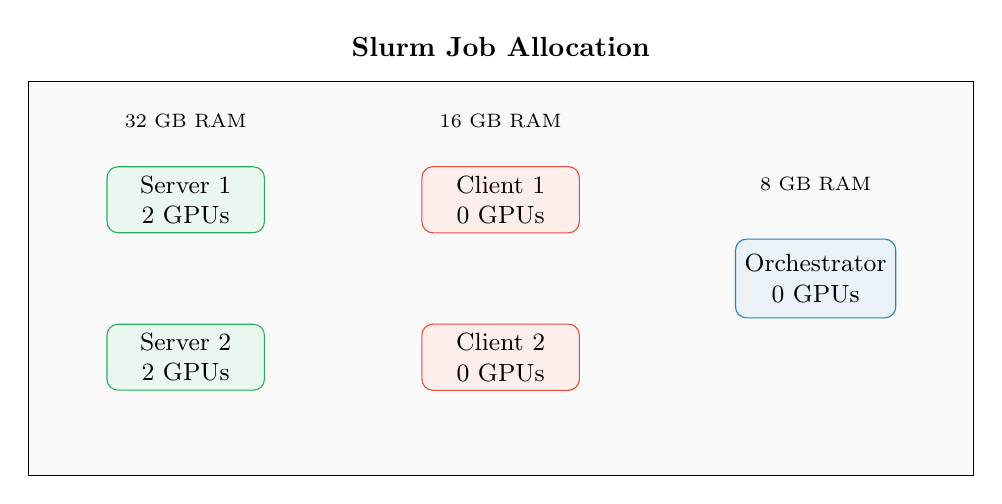
\begin{tikzpicture}[node distance=1cm]
    % Slurm allocation
    \node[draw, minimum width=12cm, minimum height=5cm, fill=gray!5] (slurm) at (0, 0) {};
    \node[above] at (0, 2.7) {\textbf{Slurm Job Allocation}};

    % Nodes
    \node[server, minimum width=2cm, align=center] (s1) at (-4, 1) {Server 1\\2 GPUs};
    \node[server, minimum width=2cm, align=center] (s2) at (-4, -1) {Server 2\\2 GPUs};
    \node[client, minimum width=2cm, align=center] (c1) at (0, 1) {Client 1\\0 GPUs};
    \node[client, minimum width=2cm, align=center] (c2) at (0, -1) {Client 2\\0 GPUs};
    \node[component, minimum width=2cm, align=center] (orch) at (4, 0) {Orchestrator\\0 GPUs};

    % Labels
    \node[font=\scriptsize] at (-4, 2) {32 GB RAM};
    \node[font=\scriptsize] at (0, 2) {16 GB RAM};
    \node[font=\scriptsize] at (4, 1.2) {8 GB RAM};
\end{tikzpicture}
\caption{Slurm resource allocation example}
\end{figure}

% ============================================================================
\section{Extensibility}
% ============================================================================

\subsection{Adding a New Service}

To add a new inference service, implement four components:

\begin{enumerate}
    \item \textbf{Server Manager}: Handle service lifecycle
    \item \textbf{Workload Controller}: Coordinate clients
    \item \textbf{Workload Executor}: Execute benchmarks
    \item \textbf{Service Registration}: Register with factory
\end{enumerate}

\begin{figure}[H]
\centering
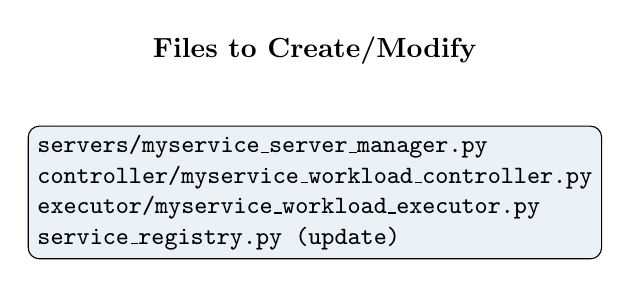
\begin{tikzpicture}[node distance=2cm]
    % Files to create
    \node[draw, rounded corners, fill=primary!10, minimum width=6cm, align=left, font=\small\ttfamily] (files) at (0, 0) {
        servers/myservice\_server\_manager.py \\
        controller/myservice\_workload\_controller.py \\
        executor/myservice\_workload\_executor.py \\
        service\_registry.py (update)
    };

    \node[above] at (0, 1.5) {\textbf{Files to Create/Modify}};
\end{tikzpicture}
\end{figure}

\subsection{Custom Metrics}

Extend the Monitor class for custom metrics:

\begin{lstlisting}[style=python, caption={Custom metrics extension}]
from prometheus_client import Gauge

class CustomMonitor(Monitor):
    def __init__(self, *args, **kwargs):
        super().__init__(*args, **kwargs)
        self.custom_metric = Gauge(
            'custom_metric',
            'Description of custom metric'
        )

    def collect_custom(self):
        value = self._get_custom_value()
        self.custom_metric.set(value)
\end{lstlisting}

% ============================================================================
\section{Deployment and Operations}
% ============================================================================

\subsection{Prerequisites}

\begin{table}[H]
\centering
\begin{tabular}{@{}lll@{}}
\toprule
\textbf{Component} & \textbf{Requirement} & \textbf{Version} \\
\midrule
Python & Runtime & 3.6+ \\
Slurm & Job scheduler & Any \\
Apptainer & Container runtime & 1.0+ \\
Docker & Local monitoring & 20.10+ \\
\bottomrule
\end{tabular}
\caption{System prerequisites}
\end{table}

\subsection{Python Dependencies}

\begin{lstlisting}[style=bash, caption={Required Python packages}]
pip install flask requests psutil prometheus_client pyyaml
\end{lstlisting}

\subsection{Container Setup}

\begin{lstlisting}[style=bash, caption={Building containers on MeluXina}]
module load Apptainer

# Pull Ollama container
apptainer pull docker://ollama/ollama:latest

# Pull vLLM container
apptainer pull docker://vllm/vllm-openai:latest

# Pull Python container for clients
apptainer pull docker://python:3.12.3-slim
\end{lstlisting}

% ============================================================================
\section{Troubleshooting Guide}
% ============================================================================

\subsection{Common Issues}

\begin{table}[H]
\centering
\begin{tabular}{@{}p{4cm}p{4cm}p{6cm}@{}}
\toprule
\textbf{Issue} & \textbf{Symptom} & \textbf{Solution} \\
\midrule
Server health check fails & Timeout during startup & Verify port accessibility, check container logs \\
Client cannot connect & Connection refused & Check executor is running, verify port \\
No metrics in Grafana & Empty dashboard & Verify SSH tunnel, check Prometheus targets \\
Ray cluster fails & Workers not connecting & Check network ports, verify head IP \\
\bottomrule
\end{tabular}
\caption{Common issues and solutions}
\end{table}

\subsection{Debugging Commands}

\begin{lstlisting}[style=bash, caption={Useful debugging commands}]
# Check server health
curl http://server-node:11434/api/tags

# Verify executor
curl http://client-node:6000/health

# Check Prometheus targets
curl http://localhost:9092/api/v1/targets

# View Ray cluster status
ssh head-node "ray status"
\end{lstlisting}

% ============================================================================
\section{Project Structure}
% ============================================================================

\begin{lstlisting}[style=bash, caption={Complete project structure}]
hpc-benchmark-toolkit/
+-- src/
|   +-- benchmark/
|   |   +-- orchestrator.py
|   |   +-- service_factory.py
|   |   +-- service_registry.py
|   |   +-- servers/
|   |   |   +-- base_server_manager.py
|   |   |   +-- ollama_server_manager.py
|   |   |   +-- vllm_server_manager.py
|   |   |   +-- ray_cluster_manager.py
|   |   +-- workload/
|   |   |   +-- controller/
|   |   |   +-- executor/
|   |   +-- logging/
|   +-- benchmark_cli.py
|   +-- monitor/
|       +-- monitor.py
+-- monitoring/
|   +-- docker-compose.yml
|   +-- prometheus.yml
|   +-- grafana/
+-- schemas/
|   +-- recipe-format.yaml
+-- docs/
+-- diagrams/
\end{lstlisting}

% ============================================================================
\section{Division of Work}
% ============================================================================

This section documents the contributions of each team member to the project.

\subsection{Alberto Finardi}

\textbf{Role}: System Architect, Infrastructure, and Core Implementation\\
\textbf{Contributions}:
\begin{itemize}
    \item \textbf{Core Infrastructure}
    \begin{itemize}
        \item Designed and implemented the overall system architecture
        \item Created the Service Factory pattern for extensibility
        \item Built the modular component structure
        \item Implemented service registry for dynamic component loading
    \end{itemize}

    \item \textbf{Server Management}
    \begin{itemize}
        \item Implemented \texttt{BaseServerManager} abstract class
        \item Developed \texttt{OllamaServerManager} with health checks and model pulling
        \item Developed \texttt{VllmServerManager} with distributed support
        \item Created \texttt{RayClusterManager} for distributed vLLM deployments
    \end{itemize}

    \item \textbf{Workload Controllers}
    \begin{itemize}
        \item Designed \texttt{BaseWorkloadController} interface
        \item Implemented service-specific controllers (Ollama, vLLM)
        \item Developed HTTP-based client coordination protocol
    \end{itemize}

    \item \textbf{Workload Executors}
    \begin{itemize}
        \item Created \texttt{BaseWorkloadExecutor} Flask server framework
        \item Implemented REST API endpoints for workload management
        \item Developed thread pool management for concurrent requests
        \item Built metrics collection infrastructure
    \end{itemize}

    \item \textbf{Benchmarking Framework}
    \begin{itemize}
        \item Implemented core benchmarking logic
        \item Developed request generation and load patterns
        \item Created latency measurement and metrics aggregation
        \item Built Ollama and vLLM specific benchmark implementations
    \end{itemize}

    \item \textbf{CLI Development}
    \begin{itemize}
        \item Developed \texttt{benchmark\_cli.py} with three main commands
        \item Implemented interactive recipe creation wizard
        \item Created deployment and job submission logic
        \item Built recipe listing and management features
    \end{itemize}

    \item \textbf{Orchestration}
    \begin{itemize}
        \item Implemented main orchestrator logic (\texttt{orchestrator.py})
        \item Developed seven-phase execution model
        \item Created Slurm sbatch script generation
        \item Built node allocation and resource management
    \end{itemize}

    \item \textbf{Basic Logging Infrastructure}
    \begin{itemize}
        \item Set up initial logging framework
        \item Implemented basic log output and formatting
        \item Created log directory structure
    \end{itemize}

    \item \textbf{Documentation}
    \begin{itemize}
        \item Wrote comprehensive README.md
        \item Created API Reference documentation
        \item Developed Developer Guide
        \item Authored this technical report
    \end{itemize}

    \item \textbf{Integration}
    \begin{itemize}
        \item Integrated all team contributions
        \item Coordinated component interfaces
        \item Performed system testing and debugging
    \end{itemize}
\end{itemize}

\subsection{Giovanni}

\textbf{Role}: Monitoring Integration\\
\textbf{Contributions}:
\begin{itemize}
    \item \textbf{Prometheus Integration}
    \begin{itemize}
        \item Configured Prometheus for metrics collection
        \item Set up Docker container for Prometheus server
    \end{itemize}

    \item \textbf{Grafana Dashboards}
    \begin{itemize}
        \item Created Grafana dashboards for Ollama and vLLM metrics visualization
        \item Configured Docker container for Grafana
    \end{itemize}
\end{itemize}

\subsection{Laura}

\textbf{Role}: Recipe Validation and Benchmark Execution\\
\textbf{Contributions}:
\begin{itemize}
    \item \textbf{Recipe Validation System}
    \begin{itemize}
        \item Designed JSON Schema for recipe validation (\texttt{schemas/recipe-format.yaml})
        \item Implemented validation logic and error handling
        \item Created custom validators for service-specific configurations
        \item Developed user-friendly error message formatting
        \item Built schema versioning support
    \end{itemize}

    \item \textbf{Benchmark Execution}
    \begin{itemize}
        \item Ran and validated Ollama benchmarks on MeluXina
        \item Ran and validated vLLM benchmarks (single and distributed)
        \item Tested parameter sweep configurations
        \item Verified metrics collection and reporting
    \end{itemize}

    \item \textbf{Documentation}
    \begin{itemize}
        \item Recipe validation section of this report
        \item Benchmarking implementation section of this report
    \end{itemize}
\end{itemize}

\subsection{Giulia}

\textbf{Role}: Logging System\\
\textbf{Contributions}:
\begin{itemize}
    \item \textbf{Logging Architecture}
    \begin{itemize}
        \item Designed overall logging architecture
        \item Defined log sources and destinations
        \item Created aggregation strategy for distributed logs
    \end{itemize}

    \item \textbf{BaseLogCollector}
    \begin{itemize}
        \item Implemented abstract interface for log collection
        \item Designed \texttt{LogSource} dataclass
        \item Defined method specifications for collectors
    \end{itemize}

    \item \textbf{TailerLogCollector}
    \begin{itemize}
        \item Implemented file tailing for real-time log collection
        \item Built remote node log collection via SSH
        \item Created log aggregation from multiple sources
    \end{itemize}

    \item \textbf{Log Management}
    \begin{itemize}
        \item Implemented structured logging format (JSON)
        \item Added timestamps and correlation IDs
        \item Organized storage structure
        \item Defined retention policies
    \end{itemize}

    \item \textbf{Documentation}
    \begin{itemize}
        \item Logging system section of this report
    \end{itemize}
\end{itemize}

\subsection{Contribution Summary}

\begin{table}[H]
\centering
\begin{tabular}{@{}llp{6cm}@{}}
\toprule
\textbf{Team Member} & \textbf{Primary Area} & \textbf{Key Deliverables} \\
\midrule
Alberto Finardi & Infrastructure \& Core & Orchestrator, Server Managers, Controllers, Executors, Benchmarks, CLI, Basic Logging, Documentation \\
Giovanni & Monitoring & Prometheus/Grafana integration, Dashboards \\
Laura & Validation & Recipe validation, Benchmark execution \\
Giulia & Logging & Log collectors, Aggregation \\
\bottomrule
\end{tabular}
\caption{Team contribution summary}
\end{table}

% ============================================================================
\section{Conclusion}
% ============================================================================

The HPC Benchmark Toolkit provides a comprehensive solution for benchmarking LLM inference services on HPC clusters. Key achievements include:

\begin{itemize}
    \item \textbf{Modular Architecture}: Clean separation of concerns with factory pattern
    \item \textbf{Multi-Service Support}: Ollama, vLLM (single and distributed)
    \item \textbf{Real-Time Monitoring}: Full Prometheus/Grafana integration
    \item \textbf{Reproducibility}: YAML-based recipe system
    \item \textbf{Extensibility}: Easy addition of new services
    \item \textbf{HPC Integration}: Native Slurm and Apptainer support
\end{itemize}

\subsection{Future Work}

Potential enhancements include:
\begin{itemize}
    \item Support for additional inference services (TensorRT, Triton)
    \item Kubernetes orchestration mode
    \item Automated performance regression testing
    \item Interactive web dashboard
    \item Multi-cluster support
\end{itemize}

% ============================================================================
% Appendices
% ============================================================================

\appendix

\section{Port Reference}

\begin{table}[H]
\centering
\begin{tabular}{@{}lll@{}}
\toprule
\textbf{Port} & \textbf{Service} & \textbf{Description} \\
\midrule
11434 & Ollama & Default Ollama API \\
8000 & vLLM & Default vLLM API \\
5000/6000 & Executor & Workload executor Flask \\
9091 & Pushgateway & Prometheus Pushgateway \\
9092 & Prometheus & Prometheus server \\
3001 & Grafana & Grafana dashboard \\
6379 & Ray & Ray cluster communication \\
8265 & Ray Dashboard & Ray monitoring \\
8076 & Ray Object Manager & Ray object store \\
8077 & Ray Node Manager & Ray node management \\
\bottomrule
\end{tabular}
\caption{Complete port reference}
\end{table}

\section{Environment Variables}

\begin{table}[H]
\centering
\begin{tabular}{@{}lll@{}}
\toprule
\textbf{Variable} & \textbf{Description} & \textbf{Default} \\
\midrule
PYTHONPATH & Python module path & -- \\
MLUX\_USER & MeluXina username & -- \\
MLUX\_ACCOUNT & MeluXina project account & -- \\
MLUX\_KEY & Path to SSH key & \textasciitilde/.ssh/id\_ed25519\_mlux \\
\bottomrule
\end{tabular}
\caption{Environment variables}
\end{table}

\end{document}
